\chapter[
     image=cap3,%genetics-dogs,
     image caption={The global option open right, triggers the typesetting of chapter on odd pages only. There are a  couple of layouts that must be typeset on an even pages.}]%
         %{1}
{Definiciones y construcciones}
{\hspace*{20pt} La geometr\'{\i}a nace de la necesidad de los antiguos Egipcios en medir sus
tierras despu\'{e}s de una inundaci\'{o}n del río Nilo, luego los griegos la
convirtieron en una disciplina hasta cuando Euclides la organiz\'{o} \
convirtiéndola en la primera rama de las matem\'{a}ticas que fue
axiomatizada.
Decir que la geometr\'{\i}a fue axiomatizada, quiere decir que tiene una
estructura de la siguiente forma:

\begin{itemize}
\item Lo primero es establecer un conjunto mínimo de t\'{e}rminos, los cuales no se
pueden definir, pero que de forma natural se pueden conocer sus caracter%
\'{\i}sticas o propiedades.

\item A partir de los elementos anteriores se construyen otros usando
proposiciones en forma de equivalencia. estas proposiciones se llaman
definiciones.

\item Luego se establecen un conjunto de propiedades independientes,\ los cuales son
ciertos por si solos , es decir su validez es evidente. A este conjunto de
propiedades se llaman axiomas y/o postulados.

\item Para terminar se construyen a partir de todo lo anterior un conjunto
ilimitado de propiedades, las cuales no son evidentes por si solas y por lo
tanto es necesario demostrarlas a partir de proposiciones verdaderas usando
los m\'{e}todos de demostraci\'{o}n establecidos por la lógica.
\end{itemize}
  }
\label{chap:1}
\seccion{Términos}
\label{sec:1.1}
 Antes de empezar la construcción de la geometría estableceremos alguna ideas generales.\\
Por ejemplo:
\begin{ideas}{Término es una palabra o propiedad que representa a un elemento o la relación entre varios elementos. }{}
\end{ideas}

\begin{ideas}{ Cantidad es cualquier objeto y/o fenómeno que puede ser medida, es decir,
medir un objeto es encontrar cuántas veces contiene un patrón del mismo tipo al objeto.
A ese patrón tomado como estándar. Se llama  unidad de medida.
}{Cantidad}
En \texttt{GEOMETRÍA} hay cuatro especies de cantidades, \texttt{LÍNEAS,
SUPERFICIES, VOLUMEN y
ÁNGULOS}. Estas son llamadas \underline{MAGNITUDES GEOMÉTRICAS}.
Dado que la unidad de medida de una cantidad es del mismo tipo que la cantidad
medida, hay cuatro tipos de unidades de medición: unidades de \textbf{longitud}, unidades
de \textbf{superficie}, unidades de \textbf{volumen} y unidades de \textbf{medida angular}. \\
Basandonos en la anterior idea podemos establecer lo que es la geometría.
\begin{ideas}{GEOMETRÍA es la rama de las matemáticas que estudia las propiedades, relaciones y
medidas de las magnitudes geométricas.
}{Geometría}
En Geometría, las medidas de las cantidades consideradas son generalmente representadas por
medio de letras minúsculas. Las operaciones a realizarse con las medidas de las cantidades
y las relaciones entre ellas, son las establecidas por el \textbf{álgebra}.
Si $a$ y $b$ son medidas de  cantidades geométricas, se tiene:
\begin{lista}
 \item La operación \textbf{adición} , la cual usa el signo llamado más, $+$;
 Entonces, $a + b$ indica que $b$ y $a$ son sumados.
\item La operación \textbf{substracción}, la cual usa el signo llamado menos, $-$ ;
Entonces, $a-b$ indica que $b$ es el sustraendo y $a$ el minuendo.
\item La operación \textbf{multiplicación o producto},la cual usa el signo llamado por, $\cdot$ ;
Entonces, $a \cdot b$ indica que $a$ y $b$ son factores.
\item La operación \textbf{división}, la cual usa el signo $/$, llamado entre;
Entonces, $a/b$, indica que $b$ es el divisor y $a$ el dividendo.
\item La \textbf{potenciación} $a^n$ , indica que $a$ se tomará $n$ veces como factor,
 o elevado a la enésima potencia,\, \nota \, $a\neq 0$ y $n \in \mathbb{N}$.
\item La \textbf{radicación} $\sqrt[n]{a}$, indica que existe
 un $b \in \mathbb{R}$ tal que  $b^n=a$ .
\item La relación \textbf{igualdad} $a=b$,
lo que significa que $a-b$ es $0$.
\item La relación \textbf{menor que} $a<b$,
 lo que significa que $a-b \in \mathbb{R^-}$.
\item La relación \textbf{mayor que} $a>b$,
lo que significa que $a-b \in \mathbb{R^+}$.
\item La relación \textbf{menor o igual} $a\leq b$, lo que significa que $a=b$ o $a<b$,
\item La relación \textbf{mayor o igual} $a\geq b$, lo que significa que $a=b$ o $a>b$,
\end{lista}
En todos los casos las medidas de las cantidades geométricas son números reales no negativos.\\
\nota \, Estudiar las propiedades de las operaciones y las relaciones de los
números reales en el apéndice A.
\end{ideas}
\begin{ideas}{Una \textbf{proposición} es un enunciado al cual se le puede asignar un valor de verdad,
es decir puede ser falso o verdadero, pero no ambas.}{Proposición}
Por ejemplo:
\begin{lista}
 \item $3+2=5$. De acuerdo con la definición de adición entre naturales,
este enunciado es verdadero, por lo tanto es una proposición.
\item Mañana llueve. esto es algo que no se puede saber antes de termine el día, por lo tanto
no se le puede asignar un valor de verdad, es decir este enunciado no es una proposición.
\end{lista}
\begin{ideas}{Una \textbf{tautología} es una proposición que siempre es
verdadera. }{Tautología}
 A las tautologías a veces en geometría se les llama verdades geométricas o afirmaciones.
Las verdades generales de la geometría se deducen a partir del razonamiento lógico,
siendo las premisas definiciones, postulados o principios previamente
establecidos. El razonamiento utilizado para establecer cualquier verdad o
principio es llamado una demostración.
\end{ideas}
\begin{ideas}{Una \textbf{definición} es una afirmación que explica el significado de un término o una palabra, en función
de palabras o términos conocidos.}{Definición}
En caso de que un término no se pueda expresar en función de otros términos ya establecidos, se dice que es un término no definido.
\end{ideas}
\begin{ideas}{Un \textbf{teorema} es una verdad que requiere demostración.}{Teorema}
 \end{ideas}
\begin{ideas}{Un \textbf{axioma} es una verdad auto-evidente.}{Axioma}
Un \textbf{PROBLEMA} es una situación o proposición que requiere solución.
 \end{ideas}
\begin{ideas}{Un \textbf{Postulado} es un problema auto-evidente.}{Postulado}
\end{ideas}
\begin{ideas}{Una \textbf{hipótesis} es una suposición hecha, bien en el texto
de una proposición, o en el
curso de una demostración.
}{Hipótesis}
\end{ideas}
\end{ideas}
\end{ideas}
\seccion{T\'{e}rminos no definidos}
\label{sec:1.2}
En geometr\'{\i}a tenemos que utilizar algunos elementos que no podemos
definir, lo que podemos hacer es tener una idea de lo que son. Estos
elementos son; el punto, la linea recta y el plano.
Un punto lo representa la marca que deja un l\'{a}piz de punta muy fina en
una hoja de papel.
\begin{tndefinido}{Podemos decir que representa un punto, no lo que es un punto:

Un punto lo representa la marca que deja un l\'{a}piz de punta muy fina en
una hoja de papel.}{El Punto}
 Los punto se denotan con letras may\'{u}sculas, generalmente las primeras
del alfabeto. por ejemplo: \\
\definecolor{qqqqff}{rgb}{0,0,1}
\begin{figure}[H]
\centering
 \begin{tikzpicture}[scale=0.7,font=\fontsize{7}{7}\selectfont,line cap=round,line join=round,>=triangle 45,x=1.0cm,y=1.0cm]
\clip(1.4,-1.76) rectangle (5.68,2.06);
\fill [color=qqqqff] (1.86,1.6) circle (1.5pt);
\draw[color=qqqqff] (2.02,1.86) node {$A$};
\fill [color=qqqqff] (4.86,0.54) circle (1.5pt);
\draw[color=qqqqff] (5,0.8) node {$B$};
\fill [color=qqqqff] (3.1,-0.7) circle (1.5pt);
\draw[color=qqqqff] (3.08,-0.94) node {$C$};
\end{tikzpicture}
\caption{Los puntos $A$,$B$ y $C$}
\label{fig1}
\end{figure}
\end{tndefinido}
\begin{tndefinido}{Una linea recta la representa una cuerda delgada y tensa la cual es
infinitamente larga.}{Linea Recta}
Las rectas se denotan con letras min\'{u}sculas, generalmente a partir de la
$l$ tambi\'{e}n podemos tomar dos puntos sobre ella como por ejemplo:
\begin{figura}{\definecolor{qqqqff}{rgb}{0,0,1}
\begin{tikzpicture}[scale=0.7,font=\fontsize{7}{7}\selectfont,line cap=round,line join=round,>=triangle 45,x=1.0cm,y=1.0cm]
%\clip(-3.98,0.02) rectangle (5.08,5.06);
\draw [domain=-3.98:5.08,<->] plot(\x,{(--10.45--2.56*\x)/4.02});
\fill [color=qqqqff] (-0.94,2) circle (1.5pt);
\draw[color=qqqqff] (-1.44,2,0) node {$A$};
\fill [color=qqqqff] (3.08,4.56) circle (1.5pt);
\draw[color=qqqqff] (3.14,4.2) node {$B$};
\draw[color=black] (-2.8,1.22) node {$l$};
\end{tikzpicture}}{Linea $l$}{fig2}
La recta de la figura (\ref{fig2}) se denota: $\overleftrightarrow{AB}$ o $l$
\end{figura}
\end{tndefinido}
\begin{tndefinido}{Una buena idea de lo que es el plano es decir que lo representa una hoja de
papel delgada e infinitamente grande.}{El Plano}
 Los planos se denotan con letras g\'{o}ticas may\'{u}sculas, por ejemplo:
\vskip -40pt
\begin{figura}{\definecolor{zzttqq}{rgb}{0.6,0.2,0}
\definecolor{qqqqff}{rgb}{0,0,1}
\begin{tikzpicture}[scale=0.7,font=\fontsize{7}{7}\selectfont,line cap=round,line join=round,>=triangle 45,x=1.0cm,y=1.0cm]
\clip(-1.58,-1.98) rectangle (8.64,5.1);
\fill[color=red!5,fill=red!50,fill opacity=0.1] (-0.4,3.66) -- (-0.48,-0.4) -- (6.66,-0.4) -- (6.78,3.66) -- cycle;
% \draw [color=zzttqq] (-0.4,3.66)-- (-0.48,-0.4);
% \draw [color=zzttqq] (-0.48,-0.4)-- (6.66,-0.4);
% \draw [color=zzttqq] (6.66,-0.4)-- (6.78,3.66);
% \draw [color=zzttqq] (6.78,3.66)-- (-0.4,3.66);
\draw (6.2,3.42) node[anchor=north west] {$\xi$};
% \fill [color=qqqqff] (-0.4,3.66) circle (1.5pt);
% \draw[color=qqqqff] (-0.24,3.92) node {$A$};
% \fill [color=qqqqff] (-0.48,-0.4) circle (1.5pt);
% \draw[color=qqqqff] (-0.34,-0.60) node {$B$};
% \fill [color=qqqqff] (6.66,-0.4) circle (1.5pt);
% \draw[color=qqqqff] (6.82,-0.60) node {$C$};
% \fill [color=qqqqff] (6.78,3.66) circle (1.5pt);
% \draw[color=qqqqff] (6.94,3.92) node {$D$};
% \draw[color=zzttqq] (-0.7,1.78) node {$a$};
% \draw[color=zzttqq] (3.16,-0.58) node {$b$};
% \draw[color=zzttqq] (7.08,1.78) node {$c$};
% \draw[color=zzttqq] (3.26,4.12) node {$d$};
\end{tikzpicture}\\
}{El Plano}{fig3}
El plano $\xi$ en la figura (\ref{fig3}).\\ \nota \, Observe que la figura (\ref{fig3}) no tiene bordes,
 lo cual significa  que es ilimitado.
\end{figura}
\end{tndefinido}
\vspace*{20pt}
\seccion{Definiciones preliminares}
\label{sec:1.3}
Despu\'{e}s de identificar \ el punto la recta y el plano podemos definir a
partir de \\ ellos otros elementos de la geometr\'{\i}a como los que veremos en
esta secci\'{o}n. \\
\begin{definicion}{El espacio es el conjunto de todos los puntos \hfill}{El Espacio}
De la definici\'{o}n podemos deducir que el espacio es un ente abstracto
pero que existe porque por lo menos podemos construir un punto y este punto
estar\'{\i}a en el espacio, veamos que es evidente que existen infinitos puntos y
que muchos no se encuentran en un plano por lo que es necesario hablar del
espacio.
\end{definicion}
\begin{definicion}{Un segmento de recta es un subconjunto de la linea recta determinado por dos
puntos y todos los puntos que se encuentran entre ellos.
}{Segmento de recta}
 \begin{figura}{\definecolor{qqqqff}{rgb}{0,0,1}
\begin{tikzpicture}[scale=0.7,font=\fontsize{7}{7}\selectfont,line cap=round,line join=round,>=triangle 45,x=1.0cm,y=1.0cm]
\clip(-3.14,0.66) rectangle (3.12,2.64);
\draw (-2.04,1.2)-- (1.44,1.9);
\fill [color=qqqqff] (-2.04,1.2) circle (1.5pt);
\draw[color=qqqqff] (-2.32,1.7) node {$A$};
\fill [color=qqqqff] (1.44,1.9) circle (1.5pt);
\draw[color=qqqqff] (1.44,2.52) node {$B$};
\end{tikzpicture}}{Segmento de recta}{seg}
 Notaci\'{o}n: Sean $A$ y $B$ dos puntos de una recta, el segmento
determinado por ellos se denota como $\overline{AB}$ . A los puntos $A$ y $B$
se les lama extremos del segmento
 \end{figura}
\end{definicion}
\begin{definicion}{Los puntos de un conjunto se dice que est\'{a}n alineados o son co\-li\-nea\-les
si existe una recta que los contiene a todos.}{Puntos colineales}
\begin{figura}{\definecolor{xdxdff}{rgb}{0.49,0.49,1}
\definecolor{qqqqff}{rgb}{0,0,1}
\begin{tikzpicture}[scale=0.7,font=\fontsize{7}{7}\selectfont,line cap=round,line join=round,>=triangle 45,x=1.0cm,y=1.0cm]
\clip(-3.56,-0.6) rectangle (4.28,3.18);
\draw (-2.04,1.2)-- (1.44,1.9);
\draw [domain=-3.56:4.28,<->] plot(\x,{(--5.6--0.7*\x)/3.48});
\fill [color=qqqqff] (-2.04,1.2) circle (1.5pt);
\draw[color=qqqqff] (-2.32,1.7) node {$A$};
\fill [color=qqqqff] (1.44,1.9) circle (1.5pt);
\draw[color=qqqqff] (1.44,2.52) node {$B$};
\draw[color=black] (-2.86,0.84) node {$b$};
\fill [color=xdxdff] (3.66,2.35) circle (1.5pt);
\draw[color=xdxdff] (3.54,2.88) node {$C$};
\fill [color=qqqqff] (0.24,0.3) circle (1.5pt);
\draw[color=qqqqff] (0.28,-0.04) node {$D$};
\end{tikzpicture}}{Punto Alineados}{alin}
Por ejemplo en la figura (\ref{alin}) el conjunto de puntos $\left\{ A,B,C\right\} $ es un conjunto de
puntos alineados, mientras que el conjunto de puntos $\left\{
A,B,C,D\right\} $ no es un conjunto de puntos alineados, porque el punto $D$ no está en la recta $\overrightarrow{b}$.
\end{figura}
\end{definicion}
\begin{definicion}{Los puntos de un conjunto son coplanarios si existe un plano que los
contiene a todos.}{Puntos coplanarios}
\end{definicion}
%%%%%%%%%%%%%%%%%%%%%%%%%%%%%%%%%%%%%%%%%%%%%%%%%%%%%%%%%%%%%%%%%%%%%%%%%%%%%%%%%%%%%%%%%
\begin{figura}{
\definecolor{zzttqq}{rgb}{0.6,0.2,0}
\definecolor{uququq}{rgb}{0.25,0.25,0.25}
\definecolor{qqqqff}{rgb}{0,0,1}
\definecolor{cqcqcq}{rgb}{0.75,0.75,0.75}
\begin{tikzpicture}[scale=0.7,font=\fontsize{7}{7}\selectfont,line cap=round,line join=round,>=triangle 45,x=1.0cm,y=1.0cm]
\draw [color=cqcqcq,dash pattern=on 2pt off 2pt, xstep=1.0cm,ystep=1.0cm] (-0.34,-0.14) grid (12.74,8.49);
\clip(-0.34,-0.14) rectangle (12.74,8.49);
\fill[color=zzttqq,fill=zzttqq,fill opacity=0.1] (6.09,3.75) -- (7.15,4.13) -- (7.15,4.51) -- (6.08,4.2) -- cycle;
\draw (0,1)-- (3,5);
\draw (12,5)-- (3,5);
\draw (9,1)-- (12,5);
\draw (0,1)-- (9,1);
\draw (1.4,2.12) node[anchor=north west] {$l_1$};
\draw (10.01,3.91) node[anchor=north west] {$l_2$};
\draw [color=zzttqq] (6.09,3.75)-- (7.15,4.13);
\draw [color=zzttqq] (7.15,4.13)-- (7.15,4.51);
\draw [color=zzttqq] (7.15,4.51)-- (6.08,4.2);
\draw [color=zzttqq] (6.08,4.2)-- (6.09,3.75);
\draw [line width=1.2pt,dotted] (6.09,3.75)-- (6.18,-0.54);
\draw (6,8)-- (6.09,3.75);
\draw (0.58,1.77)-- (9.57,5);
\draw (2.31,1)-- (11.52,4.37);
\fill [color=qqqqff] (0,1) circle (1.5pt);
\fill [color=qqqqff] (3,5) circle (1.5pt);
\fill [color=qqqqff] (12,5) circle (1.5pt);
\fill [color=qqqqff] (9,1) circle (1.5pt);
\fill [color=qqqqff] (3.32,3.82) circle (1.5pt);
\draw[color=qqqqff] (3.46,4.05) node {$A$};
\fill [color=qqqqff] (8.24,3.76) circle (1.5pt);
\draw[color=qqqqff] (8.38,4) node {$B$};
\fill [color=qqqqff] (7.58,1.74) circle (1.5pt);
\draw[color=qqqqff] (7.72,1.98) node {$C$};
\fill [color=qqqqff] (6,8) circle (1.5pt);
\draw[color=qqqqff] (6.14,8.22) node {$D$};
\fill [color=uququq] (6.09,3.75) circle (1.5pt);
\end{tikzpicture}}{Puntos coplanarios}{pcopl}
En la figura suponemos que el punto $D$ no está en el plano.
\end{figura}
%%%%%%%%%%%%%%%%%%%%%%%%%%%%%%%%%%%%%%%%%%%%%%%%%%%%%%%%%%%%%%
\begin{ejemplo}{La figura (\ref{pcopl}) nos muestra varios conjuntos de puntos indiquemos si son o no
coplanarios}
\solucion
\begin{itemize}
\item Las rectas $l_{1}$ y $l_{2}$ son coplanarias

\item Los puntos $A,B$ y $C$ son coplanarios

\item Los puntos $A,B,C$ y $D$ no son coplanarios

\item La recta $l_{1}$ y el punto $A$ son coplanarios

\item La recta $l_{2}$ y el punto $D$ no son coplanarios.
\end{itemize}
 \end{ejemplo}
\begin{definicion}{Son dos o mas rectas que se intersecan en un punto.}{Rectas Intersecantes}
\begin{figura}{\definecolor{qqqqff}{rgb}{0,0,1}
\begin{tikzpicture}[scale=0.7,font=\fontsize{7}{7}\selectfont,line cap=round,line join=round,>=triangle 45,x=1.0cm,y=1.0cm]
\clip(-0.61,-1.38) rectangle (11.45,7.82);
\draw [->] (3.01,-0.04) -- (7.48,6.8);
\draw [->] (2.46,6.56) -- (7.56,-0.45);
\draw [->] (9.53,4.34) -- (-0.07,1.57);
\draw [->] (5,7) -- (5.04,-0.67);
\draw [->] (3.45,0.63) -- (2.95,-0.14);
\draw [->] (8.93,4.16) -- (9.8,4.42);
\draw [->] (5.01,6) -- (5,7.22);
\draw [->] (3.07,5.73) -- (2.37,6.73);
\draw (4.88,7.74) node[anchor=north west] {$l_1$};
\draw (7.64,7.07) node[anchor=north west] {$l_2$};
\draw (9.93,4.74) node[anchor=north west] {$l_3$};
\draw (7.62,-0.34) node[anchor=north west] {$l_4$};
\fill [color=qqqqff] (5.02,3.04) circle (2.0pt);
\draw[color=qqqqff] (5.39,2.89) node {$A$};
\end{tikzpicture}}{rectas Intersecantes}{recti}
\end{figura}
La intersección de las  rectas $l_1$,$l_2$,$l_3$ y $l_4$ en la figura (\ref{recti}) es el punto $A$, por lo tanto son intersecantes
\end{definicion}
\begin{definicion}{Dos recta son paralelas si y s\'{o}lo si son coplanarias y no son
intersecantes}{Rectas Paralelas}
\vskip -40pt
\begin{figura}{
\definecolor{qqqqff}{rgb}{0,0,1}
\begin{tikzpicture}[scale=0.7,font=\fontsize{7}{7}\selectfont,scale=0.6,line cap=round,line join=round,>=triangle 45,x=1.0cm,y=1.0cm]
%\clip(-3.9,-3.44) rectangle (7.76,5.8);
\draw [domain=-3.9:7.76,<->] plot(\x,{(--11.91--4.88*\x)/6.92});
\draw [domain=-3.9:7.76,<->] plot(\x,{(-13.5--4.88*\x)/6.92});
\fill [color=qqqqff] (-2.44,0) circle (1.5pt);
\draw[color=qqqqff] (-2.6,0.42) node {$A$};
\fill [color=qqqqff] (4.48,4.88) circle (1.5pt);
\draw[color=qqqqff] (4.6,4.58) node {$B$};
\draw[color=black] (-2.72,-0.48) node {$a$};
\fill [color=qqqqff] (2.54,-0.16) circle (1.5pt);
\draw[color=qqqqff] (2.7,-0.4) node {$C$};
\draw[color=black] (-0.76,-2.86) node {$b$};
\end{tikzpicture}
}{Rectas Paralelas}{recpar}
\end{figura}
\end{definicion}
\vskip -20pt
\begin{definicion}{Dos rectas son alabeadas si y s\'{o}lo si no son coplanarias y no se
intersecan}{Rectas alabeadas}
 \begin{figura}{
\definecolor{qqqqff}{rgb}{0,0,1}
\definecolor{zzttqq}{rgb}{0.6,0.2,0}
\begin{tikzpicture}[line cap=round,line join=round,>=triangle 45,x=1.0cm,y=1.0cm]
\clip(2.57,2.45) rectangle (11.28,8.68);
\fill[color=zzttqq,fill=zzttqq,fill opacity=0.1] (3.6,5.85) -- (5.27,4.43) -- (9.84,4.35) -- (7.45,5.85) -- cycle;
\draw [color=zzttqq] (3.6,5.85)-- (5.27,4.43);
\draw [color=zzttqq] (5.27,4.43)-- (9.84,4.35);
\draw [color=zzttqq] (9.84,4.35)-- (7.45,5.85);
\draw [color=zzttqq] (7.45,5.85)-- (3.6,5.85);
\draw [->] (5.75,5.15) -- (5.77,7.13);
\draw [->] (5.75,5.15) -- (6.67,5.65);
\draw [->] (5.75,5.15) -- (5.14,4.82);
\draw [->] (5.75,5.15) -- (6.29,4.5);
\draw [->] (5.75,5.15) -- (7.49,4.71);
\draw [->] (5.75,5.15) -- (4.51,5.46);
\draw [domain=2.57:11.28] plot(\x,{(--49.07-1.78*\x)/5.48});
\draw (7.6,5.21) node[anchor=north west] {$l_1$};
\draw (6.75,5.95) node[anchor=north west] {$l_2$};
\draw (6.42,5) node[anchor=north west] {$r$};
\draw (7.27,5.93) node[anchor=north west] {$\xi$};
\draw (9.73,5.8) node[anchor=north west] {$l$};
\fill [color=qqqqff] (5.75,5.15) circle (1.5pt);
\draw[color=qqqqff] (5.93,5.54) node {$E$};
\fill [color=qqqqff] (5.77,7.13) circle (1.5pt);
\draw[color=qqqqff] (5.9,7.39) node {$F$};
\draw[color=black] (-1.67,9.35) node {$h$};
\end{tikzpicture}
}{Rectas alabeadas}{recala}
\end{figura}
En la figura (\ref{recala} el punto $C$ no está en plano $\xi$, por lo tanto como las
rectas $l_1$ y $l_2$ no son coplanarias y no se cortan, entonces son alabeadas.
\end{definicion}
En la geometría \textbf{Euclideana} se establecen cinco postulados,
 nosotros estableceremos aquí sólo dos para facilitar el desarrollo, y en el segundo capítulo esta\-ble\-ce\-re\-mos más de
tres para facilitar la construcción. \footnote{En los ``Elementos de Euclides''
se establecen un conjunto de tres términos no definidos,132 definiciones, 5 postulados, 5 axiomas y 465 teoremas
repartidos en 13 libros. }.
\begin{postulado}{Entre los n\'{u}meros reales y los puntos de una recta se puede establecer
una co\-rres\-pon\-den\-cia biun\'{\i}voca, es decir
a cada punto de la recta le podemos asignar uno y s\'{o}lo un n\'{u}mero
real y cada n\'{u}mero real le podemos asignar uno y s\'{o}lo un punto de la
recta.}{De la regla}
\begin{figura}{\definecolor{qqqqff}{rgb}{0,0,1}
\definecolor{qqweqq}{rgb}{0,0.43,0}
\definecolor{zzttqq}{rgb}{0.6,0.2,0}
\definecolor{uququq}{rgb}{0.25,0.25,0.25}
\definecolor{cqcqcq}{rgb}{0.75,0.75,0.75}
\begin{tikzpicture}[scale=0.7,font=\fontsize{7}{7}\selectfont,line cap=round,line join=round,>=triangle 45,x=1.0cm,y=1.0cm]
\draw [color=cqcqcq,dash pattern=on 1pt off 1pt, xstep=1.0cm,ystep=1.0cm] (-0.04,-1.76) grid (10.18,2.02);
%\clip(-0.04,-1.76) rectangle (10.18,2.02);
\fill[color=zzttqq,fill=zzttqq,fill opacity=0.1] (0,0) -- (0,1) -- (10.17,1.01) -- (10.17,0) -- cycle;
\draw [line width=1.2pt,color=zzttqq] (0,0)-- (0,1);
\draw [line width=1.2pt,color=zzttqq] (0,1)-- (10.17,1.01);
\draw [line width=1.2pt,color=zzttqq] (10.17,1.01)-- (10.17,0);
\draw [line width=1.2pt,color=zzttqq] (10.17,0)-- (0,0);
\draw [color=qqweqq] (1,0)-- (1,0.3);
\draw [color=qqweqq] (2,0)-- (2,0.3);
\draw [color=qqweqq] (3,0)-- (3,0.3);
\draw [color=qqweqq] (4,0)-- (4,0.3);
\draw [color=qqweqq] (5,0)-- (5,0.3);
\draw [color=qqweqq] (6,0)-- (6,0.3);
\draw [color=qqweqq] (7,0)-- (7,0.3);
\draw [color=qqweqq] (8,0)-- (8,0.3);
\draw [color=qqweqq] (9,0)-- (9,0.3);
\draw [color=qqweqq] (10,0)-- (10,0.3);
\draw [color=qqweqq] (0,0)-- (0,0.1);
\draw [color=qqweqq] (0.1,0)-- (0.1,0.1);
\draw [color=qqweqq] (0.2,0)-- (0.2,0.1);
\draw [color=qqweqq] (0.3,0)-- (0.3,0.1);
\draw [color=qqweqq] (0.4,0)-- (0.4,0.1);
\draw [color=qqweqq] (0.5,0)-- (0.5,0.1);
\draw [color=qqweqq] (0.6,0)-- (0.6,0.1);
\draw [color=qqweqq] (0.7,0)-- (0.7,0.1);
\draw [color=qqweqq] (0.8,0)-- (0.8,0.1);
\draw [color=qqweqq] (0.9,0)-- (0.9,0.1);
\draw [color=qqweqq] (1,0)-- (1,0.1);
\draw [color=qqweqq] (1.1,0)-- (1.1,0.1);
\draw [color=qqweqq] (1.2,0)-- (1.2,0.1);
\draw [color=qqweqq] (1.3,0)-- (1.3,0.1);
\draw [color=qqweqq] (1.4,0)-- (1.4,0.1);
\draw [color=qqweqq] (1.5,0)-- (1.5,0.1);
\draw [color=qqweqq] (1.6,0)-- (1.6,0.1);
\draw [color=qqweqq] (1.7,0)-- (1.7,0.1);
\draw [color=qqweqq] (1.8,0)-- (1.8,0.1);
\draw [color=qqweqq] (1.9,0)-- (1.9,0.1);
\draw [color=qqweqq] (2,0)-- (2,0.1);
\draw [color=qqweqq] (2.1,0)-- (2.1,0.1);
\draw [color=qqweqq] (2.2,0)-- (2.2,0.1);
\draw [color=qqweqq] (2.3,0)-- (2.3,0.1);
\draw [color=qqweqq] (2.4,0)-- (2.4,0.1);
\draw [color=qqweqq] (2.5,0)-- (2.5,0.1);
\draw [color=qqweqq] (2.6,0)-- (2.6,0.1);
\draw [color=qqweqq] (2.7,0)-- (2.7,0.1);
\draw [color=qqweqq] (2.8,0)-- (2.8,0.1);
\draw [color=qqweqq] (2.9,0)-- (2.9,0.1);
\draw [color=qqweqq] (3,0)-- (3,0.1);
\draw [color=qqweqq] (3.1,0)-- (3.1,0.1);
\draw [color=qqweqq] (3.2,0)-- (3.2,0.1);
\draw [color=qqweqq] (3.3,0)-- (3.3,0.1);
\draw [color=qqweqq] (3.4,0)-- (3.4,0.1);
\draw [color=qqweqq] (3.5,0)-- (3.5,0.1);
\draw [color=qqweqq] (3.6,0)-- (3.6,0.1);
\draw [color=qqweqq] (3.7,0)-- (3.7,0.1);
\draw [color=qqweqq] (3.8,0)-- (3.8,0.1);
\draw [color=qqweqq] (3.9,0)-- (3.9,0.1);
\draw [color=qqweqq] (4,0)-- (4,0.1);
\draw [color=qqweqq] (4.1,0)-- (4.1,0.1);
\draw [color=qqweqq] (4.2,0)-- (4.2,0.1);
\draw [color=qqweqq] (4.3,0)-- (4.3,0.1);
\draw [color=qqweqq] (4.4,0)-- (4.4,0.1);
\draw [color=qqweqq] (4.5,0)-- (4.5,0.1);
\draw [color=qqweqq] (4.6,0)-- (4.6,0.1);
\draw [color=qqweqq] (4.7,0)-- (4.7,0.1);
\draw [color=qqweqq] (4.8,0)-- (4.8,0.1);
\draw [color=qqweqq] (4.9,0)-- (4.9,0.1);
\draw [color=qqweqq] (5,0)-- (5,0.1);
\draw [color=qqweqq] (5.1,0)-- (5.1,0.1);
\draw [color=qqweqq] (5.2,0)-- (5.2,0.1);
\draw [color=qqweqq] (5.3,0)-- (5.3,0.1);
\draw [color=qqweqq] (5.4,0)-- (5.4,0.1);
\draw [color=qqweqq] (5.5,0)-- (5.5,0.1);
\draw [color=qqweqq] (5.6,0)-- (5.6,0.1);
\draw [color=qqweqq] (5.7,0)-- (5.7,0.1);
\draw [color=qqweqq] (5.8,0)-- (5.8,0.1);
\draw [color=qqweqq] (5.9,0)-- (5.9,0.1);
\draw [color=qqweqq] (6,0)-- (6,0.1);
\draw [color=qqweqq] (6.1,0)-- (6.1,0.1);
\draw [color=qqweqq] (6.2,0)-- (6.2,0.1);
\draw [color=qqweqq] (6.3,0)-- (6.3,0.1);
\draw [color=qqweqq] (6.4,0)-- (6.4,0.1);
\draw [color=qqweqq] (6.5,0)-- (6.5,0.1);
\draw [color=qqweqq] (6.6,0)-- (6.6,0.1);
\draw [color=qqweqq] (6.7,0)-- (6.7,0.1);
\draw [color=qqweqq] (6.8,0)-- (6.8,0.1);
\draw [color=qqweqq] (6.9,0)-- (6.9,0.1);
\draw [color=qqweqq] (7,0)-- (7,0.1);
\draw [color=qqweqq] (7.1,0)-- (7.1,0.1);
\draw [color=qqweqq] (7.2,0)-- (7.2,0.1);
\draw [color=qqweqq] (7.3,0)-- (7.3,0.1);
\draw [color=qqweqq] (7.4,0)-- (7.4,0.1);
\draw [color=qqweqq] (7.5,0)-- (7.5,0.1);
\draw [color=qqweqq] (7.6,0)-- (7.6,0.1);
\draw [color=qqweqq] (7.7,0)-- (7.7,0.1);
\draw [color=qqweqq] (7.8,0)-- (7.8,0.1);
\draw [color=qqweqq] (7.9,0)-- (7.9,0.1);
\draw [color=qqweqq] (8,0)-- (8,0.1);
\draw [color=qqweqq] (8.1,0)-- (8.1,0.1);
\draw [color=qqweqq] (8.2,0)-- (8.2,0.1);
\draw [color=qqweqq] (8.3,0)-- (8.3,0.1);
\draw [color=qqweqq] (8.4,0)-- (8.4,0.1);
\draw [color=qqweqq] (8.5,0)-- (8.5,0.1);
\draw [color=qqweqq] (8.6,0)-- (8.6,0.1);
\draw [color=qqweqq] (8.7,0)-- (8.7,0.1);
\draw [color=qqweqq] (8.8,0)-- (8.8,0.1);
\draw [color=qqweqq] (8.9,0)-- (8.9,0.1);
\draw [color=qqweqq] (9,0)-- (9,0.1);
\draw [color=qqweqq] (9.1,0)-- (9.1,0.1);
\draw [color=qqweqq] (9.2,0)-- (9.2,0.1);
\draw [color=qqweqq] (9.3,0)-- (9.3,0.1);
\draw [color=qqweqq] (9.4,0)-- (9.4,0.1);
\draw [color=qqweqq] (9.5,0)-- (9.5,0.1);
\draw [color=qqweqq] (9.6,0)-- (9.6,0.1);
\draw [color=qqweqq] (9.7,0)-- (9.7,0.1);
\draw [color=qqweqq] (9.8,0)-- (9.8,0.1);
\draw [color=qqweqq] (9.9,0)-- (9.9,0.1);
\draw [color=qqweqq] (10,0)-- (10,0.1);
\draw (8.92,0.94) node[anchor=north west] {cm};
\draw [color=qqweqq](-0.04,0.58) node[anchor=north west] {0};
\draw [color=qqweqq](0.96,0.58) node[anchor=north west] {1};
\draw [color=qqweqq](1.96,0.58) node[anchor=north west] {2};
\draw [color=qqweqq](2.97,0.58) node[anchor=north west] {3};
\draw [color=qqweqq](3.96,0.58) node[anchor=north west] {4};
\draw [color=qqweqq](4.96,0.58) node[anchor=north west] {5};
\draw [color=qqweqq](5.96,0.58) node[anchor=north west] {6};
\draw [color=qqweqq](6.96,0.58) node[anchor=north west] {7};
\draw [color=qqweqq](7.96,0.58) node[anchor=north west] {8};
\draw [color=qqweqq](8.96,0.58) node[anchor=north west] {9};
%\draw [color=qqweqq](10.0,0.58) node[anchor=north west] {10};
\draw [domain=-0.04:10.18,<->] plot(\x,{(-8-0*\x)/8});
\fill [color=uququq] (0,0) circle (1.5pt);
\fill [color=qqqqff] (1,-1) circle (1.5pt);
\draw[color=qqqqff] (1.12,-1.20) node {$A$};
\fill [color=qqqqff] (9,-1) circle (1.5pt);
\draw[color=qqqqff] (8.88,-1.20) node {$B$};
\end{tikzpicture}
}{Postulado de la regla}{posreg}
En la figura (\ref{posreg}) de acuerdo con el postulado de la regla, al punto $A$
se le asigna el número $1$ y al punto $B$ se le asigna el número $9$.
 \end{figura}
 La anterior correspondencia lo tomaremos como un postulado, porque no
podemos garantizar que a cada punto le corresponde un n\'{u}mero natural,
pero parece ser evidente que si le corresponde un número real.
\end{postulado}
\begin{definicion}{Al n\'{u}mero que la anterior correspondencia \ le asigna a un punto de la
recta se le llama coordenada del punto}{Coordenada de un punto}
 Por ejemplo en la figura (\ref{posreg}) $1$ es la coordenada del punto $A$ y se denota: $A(1)$
que se lee el punto $A$ con coordenada $1$.
\end{definicion}
\begin{ejemplo}{Sean $A$ y $B$ dos puntos de una recta y sean $a$ y $b$ los n\'{u}meros
reales que la relaci\'{o}n biun\'{\i}voca le asigna a los puntos entonces
denotamos $A\left( a\right) $ y $B\left( b\right) $ para indicar que $a$ y $%
b $ son las coordenadas de los puntos $A$ y $B$}
 \end{ejemplo}
\begin{definicion}{ Sea $a$ un n\'{u}mero real se define el valor absoluto de $a~\ (\left\vert
a\right\vert )$ como:%
\begin{equation*}
\left\vert a\right\vert =\left\{
\begin{array}{cc}
-a, & \text{si }a\leq 0 \\
a, & \text{ si }a>0%
\end{array}%
\right.
\end{equation*}}{Valor absoluto}
 \end{definicion}
\begin{ejemplo}{ Calcular $\left\vert -3\right\vert $}
 \solucion \, al aplicar la definición de valor absoluto tenemos que como $a=-3<0$, entonces $\left\vert -3\right\vert =-\left( -3\right) =3$.
\end{ejemplo}
\begin{ejemplo}{Calcular $\left\vert \sqrt{2}\right\vert$}
\solucion \, si aplicamos la definición de valor absoluto obtenemos que si  $a=\sqrt{2}>0$, entonces $\left\vert \sqrt{2}\right\vert =\sqrt{2}$.
\end{ejemplo}
\begin{definicion}{Sean $A\left( a\right) $ y $B\left( b\right) $ dos puntos sobre una recta,
la distancia entre los puntos $A$ y $B$ se define:%
\begin{equation*}
AB=\left\vert b-a\right\vert
\end{equation*}}{Distancia entre dos puntos de una recta}
 \begin{ejemplo}{Calcular la distancia entre los puntos $A$ y $B$ de la figura (\ref{posreg})}
  \solucion\, Del postulado de la regla obtenemos $A(1)$ y $B(9$, así de acuerdo
con la definición de la
distancia entre dos puntos obtenemos $AB=|9cm-1cm|= 8cm$.
  \end{ejemplo}
\begin{ejemplo}{Calcule la longitud de $\overline{AB}$}
 \begin{center}
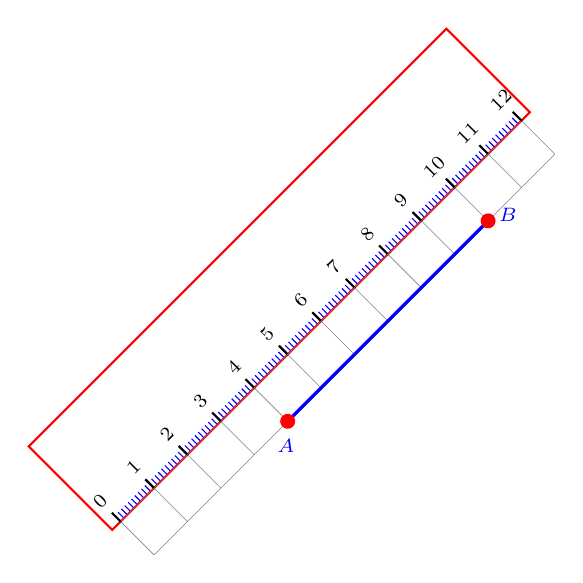
\begin{tikzpicture}[scale=0.6,font=\fontsize{7}{7}\selectfont,rotate=45]
% La regla de plastico
\draw[thick,red] (-0.25,0.0) rectangle (12.25,2.5);
% Marcas de milímetros
\foreach \x in{0.0, 0.1,...,12.0}
	\draw[blue,shift={(\x,0)}] (0,0.5pt) -- (0,5pt);
% Marcas de centímetros	
\foreach \x in{0, 1, ..., 12}
	\draw[thick,shift={(\x,0)}] (0,-0.5pt) -- (0,7.5pt) node[above,rotate=45]{$\x$};
\draw [help lines] (0,-1) grid (12,0);
\draw[blue, line width=1.2pt] (4,-1) - -  (10,-1);
\draw[color=blue,rotate=-45] (3.5,1.6) node {$A$};
\fill [color=red] (4,-1) circle (4.5pt);
\draw[color=blue,rotate=-45] (8.2,6.5) node {$B$};
\fill [color=red] (10,-1) circle (4.5pt);
\end{tikzpicture}
\end{center}
\end{ejemplo}

\end{definicion}
\begin{ejemplo}{Sean $A\left( 3\unit{cm}\right) $ y $B\left( -6\unit{cm}\right) $ dos puntos
de una recta $l$ calcule la distancia entre $A$ y $B$}
\solucion Si aplicamos la definici\'{o}n \ de distancia obtenemos%
\begin{equation*}
AB=\left\vert -6\unit{cm}-3\unit{cm}\right\vert =9\unit{cm}
\end{equation*}
\end{ejemplo}
\begin{definicion}{Sean $A\left( a\right) $ y $B\left( b\right) $ los extremos del segmento $%
\overline{AB}$ se define la longitud o medida del segmento, como la distancia entre
sus extremos
\begin{equation*}
m\overline{AB}=\left\vert b-a\right\vert
\end{equation*}}{Longitud de un segmento de recta}
\end{definicion}
\begin{ideas}{Dos objetos o elementos son congruentes si y sólo sí
tienen la misma forma y el mismo Tamaño}{Objetos congruentes}
también podemos decir que dos objetos son congruentes si al sobreponer uno sobre el otro
los dos coniciden exactamente.
 \end{ideas}

\begin{definicion}{Dos segmentos son congruentes si y sólo si tienen la misma
longitud o medida.}{Segmentos congruentes}
\end{definicion}
\begin{definicion}{El conjunto de puntos que est\'{a}n a la misma distancia de un punto fijo,
se llama circunferencia}{Circunferencia}
 \begin{figura}{\definecolor{ffqqtt}{rgb}{1,0,0.2}
\definecolor{xdxdff}{rgb}{0.49,0.49,1}
\definecolor{qqqqff}{rgb}{0,0,1}
\begin{tikzpicture}[font=\fontsize{7}{7}\selectfont,scale=0.6,line cap=round,line join=round,>=triangle 45,x=1.0cm,y=1.0cm]
\clip(-1.8,-4.74) rectangle (8.02,5.16);
\draw(3,0) circle (4.47cm);
\draw (3,0)-- (5,4);
\draw [->] (3,0) -- (5,4);
\draw [shift={(3,0)},color=ffqqtt]  plot[domain=1.11:1.98,variable=\t]({1*4.47*cos(\t r)+0*4.47*sin(\t r)},{0*4.47*cos(\t r)+1*4.47*sin(\t r)});
\fill [color=qqqqff] (3,0) circle (1.5pt);
\draw[color=qqqqff] (3.08,-0.3) node {$O$};
\fill [color=qqqqff] (5,4) circle (1.5pt);
\draw[color=qqqqff] (5.16,4.26) node {$P$};
\draw[color=black] (4.32,2) node {$r$};
\fill [color=xdxdff] (1.2,4.09) circle (1.5pt);
\draw[color=xdxdff] (0.88,4.52) node {$Q$};
\end{tikzpicture}}{La circunferencia}{cir}
\nota \, \textbf{Elementos de la circunferencia. }
\begin{lista}
\item Centro : Al punto fijo se le llama centro, por ejemplo el punto $O$ en la figura (\ref{cir}).

\item A la distancia entre el centro y  cualquier punto de la
circunferencia se le denomina radio, por ejemplo el radio de la figura (\ref{cir}) es $r=OP$.

\item Un subconjunto de al menos dos puntos de la circunferencia se le llama
arco, por ejemplo el subconjunto entre $P$ y $Q$ en la figura (\ref{cir}), y se denota $\arco[20pt]{PQ}$.
\end{lista}
   \end{figura}
\end{definicion}
\begin{definicion}{A un conjunto de puntos $X$\ se le llama circulo. Si dada una circunferencia de radio $r$\ y centro $O$, el conjunto de puntos $X$ cumple la siguiente condición. $OX<r$ }{Circulo.}
\begin{figura}{\definecolor{ttttff}{rgb}{0.2,0.2,1}
\definecolor{ffwwqq}{rgb}{1,0.4,0}
\definecolor{qqqqff}{rgb}{0,0,1}
\begin{tikzpicture}[line cap=round,line join=round,>=triangle 45,x=1.0cm,y=1.0cm]
\clip(-0.2,-6.98) rectangle (8.74,1.8);
\draw [line width=1.2pt,dash pattern=on 1pt off 1pt,color=ffwwqq,fill=ffwwqq,fill opacity=0.25] (4.08,-2.28) circle (3.59cm);
\draw [line width=2pt,dash pattern=on 3pt off 3pt,color=ttttff] (4.08,-2.28) circle (3.59cm);
\draw [->] (4.08,-2.28) -- (6.9,-4.51);
\draw (5.3,-2.56) node[anchor=north west] {$r$};
\begin{scriptsize}
\fill [color=qqqqff] (4.08,-2.28) circle (1.5pt);
\draw[color=qqqqff] (4.24,-2.02) node {$O$};
\fill [color=qqqqff] (4.32,-0.54) circle (1.5pt);
\draw[color=qqqqff] (4.48,-0.28) node {$X$};
\end{scriptsize}
\end{tikzpicture}
}{Circulo}{cir1}
\end{figura}
Observe que la circunferencia es el conjunto de puntos en azul y el circulo es el conjunto de puntos en rosado.
\end{definicion}
\begin{definicion}{Se dice que un punto de una recta $B$ est\'{a} entre dos puntos distintos $A
$ y $C$ si se cumple que%
\begin{equation*}
AB+BC=AC
\end{equation*}}{Estar entre}
\begin{figura}{\definecolor{xdxdff}{rgb}{0.49,0.49,1}
\definecolor{qqqqff}{rgb}{0,0,1}
\begin{tikzpicture}[scale=0.7,font=\fontsize{7}{7}\selectfont,line cap=round,line join=round,>=triangle 45,x=1.0cm,y=1.0cm]
%\clip(-2.44,-2.08) rectangle (4.46,2.96);
\draw [domain=-2.44:4.46,<->] plot(\x,{(-0.73--2.1*\x)/2.66});
\draw (-0.98,-1.12) node[anchor=north west] {$l_1$};
\fill [color=qqqqff] (-0.64,-0.78) circle (1.5pt);
\draw[color=qqqqff] (-0.32,-1) node {$A(3)$};
\fill [color=qqqqff] (2.02,1.32) circle (1.5pt);
\draw[color=qqqqff] (1.7,1.62) node {$B(7)$};
%\draw[color=black] (-4.12,-3.2) node {$a$};
\fill [color=xdxdff] (3.03,2.12) circle (1.5pt);
\draw[color=xdxdff] (3.42,1.7) node {$C(10)$};
\end{tikzpicture}}{Estar entre}{esten}
\begin{ejemplo}{Verificar que $B$ está entre $A$ y $C$.}
 \solucion al aplicar la definición de estar entre y de la distancia entre dos puntos observamos que:
\[ AB+BC=|7-3|+|10-7|= 4+3 = 7 \mbox{y} AC=|10-3|=7.\]
O sea que se cumple, por lo que podemos afirmar que $B$ está entre $A$ y $C$.
\end{ejemplo}
\end{figura}
\end{definicion}
\begin{definicion}{Sea una recta $l$ y sean $A,B$ y $X$ puntos de $l$ , el conjunto de puntos
del segmento $\overline{AB}$ y todos los puntos $X$ para los cuales \ se
cumple una y s\'{o}lo una de las dos condiciones

\begin{itemize}
\item $B$ est\'{a} entre $A$ y $X$

\item $A$ est\'{a} entre $B$ y $X$
\end{itemize}}{Rayo}
\begin{figura}{\definecolor{xdxdff}{rgb}{0.49,0.49,1}
\definecolor{qqqqff}{rgb}{0,0,1}
\begin{tikzpicture}[scale=0.7,font=\fontsize{7}{7}\selectfont,line cap=round,line join=round,>=triangle 45,x=1.0cm,y=1.0cm]
%\clip(-3.02,-0.06) rectangle (6.4,4.18);
\draw [domain=-3.02:6.4,<->] plot(\x,{(--10.5--0.04*\x)/3.42});
\draw (4.18,3.16) node[anchor=north west] {$l$};
\draw [domain=-3.02:6.4,<->] plot(\x,{(--3.38--0.04*\x)/3.42});
\draw (4.7,1) node[anchor=north west] {$l$};
\fill [color=qqqqff] (-2.48,3.04) circle (1.5pt);
\draw[color=qqqqff] (-2.48,3.38) node {$A$};
\fill [color=qqqqff] (0.94,3.08) circle (1.5pt);
\draw[color=qqqqff] (0.94,3.42) node {$B$};
%\draw[color=black] (-4.12,2.84) node {$a$};
\fill [color=xdxdff] (4,3.12) circle (1.5pt);
\draw[color=xdxdff] (3.98,3.46) node {$X$};
\fill [color=qqqqff] (1,1) circle (1.5pt);
\draw[color=qqqqff] (1.18,0.66) node {$A$};
%\draw[color=black] (-4.12,0.76) node {$b$};
\fill [color=xdxdff] (4,1.04) circle (1.5pt);
\draw[color=xdxdff] (4.16,0.64) node {$B$};
\fill [color=xdxdff] (-2.52,0.96) circle (1.5pt);
\draw[color=xdxdff] (-2.36,0.62) node {$X$};
\end{tikzpicture}}{Rayo}{rayo}
 \end{figura}
El rayo que contiene al segmento $\overline{AB}$ se denota $\overrightarrow{%
AB}$ o $\overleftarrow{AB}$ y al extremo se le llama origen

\nota\, De la definici\'{o}n de rayo podemos deducir que un punto divide a
una recta en dos rayos
\end{definicion}
\begin{definicion}{Un \'{a}ngulo es el conjunto determinado por la unión de dos
rayos de origen
com\'{u}n}{Ángulo}
\begin{lista}
 \item \textbf{V\'{e}rtice:} el v\'{e}rtice de un \'{a}ngulo es el origen de los rayos
que se intersecan
\item \textbf{Lados:} Los lados de un \'{a}ngulo son los rayos que lo forman
\item \textbf{Notación:} Sea el \'{a}ngulo formado por los rayos $\overrightarrow{BA}$ y $%
 \overrightarrow{BC}$ entonces se denota $\widehat{ABC}$ o $\widehat{A},$
 tambi\'{e}n se puede denotar con num\'{e}ros como $1$ o con letras
 griegas min\'{u}sculas, como $\alpha $
\end{lista}
\end{definicion}
\begin{figura}{}{Ángulo}{angulo}
\centering
 \definecolor{xdxdff}{rgb}{0.49,0.49,1}
\definecolor{qqqqff}{rgb}{0,0,1}
\begin{tikzpicture}[scale=0.7,font=\fontsize{7}{7}\selectfont,line cap=round,line join=round,>=triangle 45,x=1.0cm,y=1.0cm]
\clip(0.67,1.36) rectangle (7.57,6.2);
\draw [->] (2.08,4.66) -- (6.4,5.78);
\draw [->] (2.08,4.66) -- (6.42,1.98);
\draw [shift={(2.08,4.66)}] plot[domain=-0.55:0.25,variable=\t]({1*1.02*cos(\t r)+0*1.02*sin(\t r)},{0*1.02*cos(\t r)+1*1.02*sin(\t r)});
\draw (3.33,4.88) node[anchor=north west] {$\alpha$};
\draw (2.69,4.77) node[anchor=north west] {1};
\fill [color=qqqqff] (2.08,4.66) circle (1.5pt);
\draw[color=qqqqff] (1.59,4.82) node {$B$};
\fill [color=xdxdff] (4.57,5.31) circle (1.5pt);
\draw[color=xdxdff] (4.76,5.59) node {$A$};
\fill [color=xdxdff] (4.55,3.13) circle (1.5pt);
\draw[color=xdxdff] (4.74,3.41) node {$C$};
\end{tikzpicture}
\end{figura}
\begin{definicion}{Un conjunto de puntos se llama convexo si para cada par de puntos $A$ y $B$,
del conjunto, todo segmento $\overline{AB}$ est\'{a} contenido en el
conjunto. Si no se cumple est\'{a} condici\'{o}n se dice que el conjunto es
cóncavo}{Conjunto convexo}
\begin{center}
 \begin{figura}{\definecolor{zzttqq}{rgb}{0.6,0.2,0}
\definecolor{qqqqff}{rgb}{0,0,1}
\begin{tikzpicture}[scale=0.7,font=\fontsize{7}{7}\selectfont,line cap=round,line join=round,>=triangle 45,x=1.0cm,y=1.0cm]
\clip(-3.06,-0.66) rectangle (6.42,5.28);
\fill[color=zzttqq,fill=zzttqq,fill opacity=0.1] (2.08,4.66) -- (0.24,0.32) -- (5.5,0.36) -- (-2.18,3.96) -- cycle;
\draw [color=zzttqq] (2.08,4.66)-- (0.24,0.32);
\draw [color=zzttqq] (0.24,0.32)-- (5.5,0.36);
\draw [color=zzttqq] (5.5,0.36)-- (-2.18,3.96);
\draw [color=zzttqq] (-2.18,3.96)-- (2.08,4.66);
\draw (-0.64,3.66)-- (0.88,0.68);
\fill [color=qqqqff] (2.08,4.66) circle (1.5pt);
\draw[color=qqqqff] (2.24,4.92) node {$A$};
\fill [color=qqqqff] (0.24,0.32) circle (1.5pt);
\draw[color=qqqqff] (-0.08,0.14) node {$B$};
\fill [color=qqqqff] (5.5,0.36) circle (1.5pt);
\draw[color=qqqqff] (5.7,0.26) node {$C$};
\fill [color=qqqqff] (-2.18,3.96) circle (1.5pt);
\draw[color=qqqqff] (-2.38,4.26) node {$D$};
\fill [color=qqqqff] (-0.64,3.66) circle (1.5pt);
\draw[color=qqqqff] (-0.48,3.92) node {$E$};
\fill [color=qqqqff] (0.88,0.68) circle (1.5pt);
\draw[color=qqqqff] (1.02,0.94) node {$F$};
\end{tikzpicture}}{Conjunto cóncavo}{cconc}
En la figura (\ref{cconc}) vemos que en el conjunto sombreado determinado por los puntos
$A,B,C,$ y $D$ se puede construir un segmento $EF$ de tal forma que no está contenido totalmente
en él. Por que el conjunto no es convexo si no cóncavo.
\end{figura}
\end{center}
\begin{ejemplo}{La linea recta es un conjunto convexo}
 \end{ejemplo}
\begin{ejemplo}{El \'{a}ngulo divide el plano en tres conjuntos de puntos.

\begin{lista}
\item El \'{a}ngulo, el cual es un conjunto cóncavo.

\item Un conjunto convexo, el interior.

\item Un conjunto c\'{o}ncavo, el exterior.
\end{lista}
}
\end{ejemplo}
Trabajar con conjuntos c\'oncavos o convexos es a veces confuso, por lo que es mejor trabajar con conjuntos de puntos llamadas regiones planas
\begin{definicion}{Una regi\'on plana es un conjunto de puntos que cumple la siguiente condici\'on. Para cada punto $X$\ del conjunto existe un circulo centrado en $X$ tal que este est\'a contenido en el conjunto}{Regi\'on plana.}
 \begin{figura}{
\definecolor{cde8787}{RGB}{222,135,135}
\definecolor{ccccccc}{RGB}{204,204,204}

\begin{tikzpicture}[scale=0.8,y=0.8pt, x=0.8pt,yscale=-1, inner sep=0pt, outer sep=0pt]
\begin{scope}% layer1
  % path2987
  \path[fill=cde8787,opacity=0.534,line join=miter,line cap=butt,line
    width=0.800pt] (374.8129,334.5169) .. controls (373.6115,334.5169) and
    (372.4102,334.5169) .. (371.2089,334.5169) .. controls (370.8813,334.5169) and
    (370.5503,334.4706) .. (370.2260,334.5169) .. controls (369.3964,334.4859) and
    (368.7168,335.0415) .. (367.9326,335.1722) .. controls (367.6094,335.2261) and
    (367.2773,335.1722) .. (366.9497,335.1722) .. controls (366.2960,335.1722) and
    (365.6375,335.1722) .. (364.9839,335.1722) .. controls (364.6562,335.1722) and
    (364.3118,335.0686) .. (364.0010,335.1722) .. controls (363.4767,335.3470) and
    (363.8700,335.6527) .. (363.3457,335.8275) .. controls (362.9313,335.9656) and
    (362.4496,335.6893) .. (362.0352,335.8275) .. controls (361.5108,336.0022) and
    (361.9042,336.3079) .. (361.3799,336.4827) .. controls (361.1727,336.5518) and
    (360.9430,336.4827) .. (360.7246,336.4827) .. controls (360.0693,336.4827) and
    (359.4141,336.4827) .. (358.7588,336.4827) .. controls (358.2128,336.4827) and
    (357.6667,336.4827) .. (357.1206,336.4827) .. controls (357.0114,336.4827) and
    (356.9022,336.4827) .. (356.7930,336.4827) .. controls (356.6838,336.4827) and
    (356.5631,336.4339) .. (356.4654,336.4827) .. controls (356.1891,336.6209) and
    (356.1032,337.0403) .. (355.8101,337.1380) .. controls (355.6029,337.2071) and
    (355.3733,337.1380) .. (355.1548,337.1380) .. controls (354.2357,337.1380) and
    (354.0515,337.0344) .. (353.1890,337.4656) .. controls (352.6105,337.7549) and
    (351.8018,338.4869) .. (351.2232,338.7762) .. controls (350.9143,338.9306) and
    (350.5680,338.9946) .. (350.2403,339.1038) .. controls (349.5853,339.3222) and
    (348.9296,339.5407) .. (348.2745,339.7591) .. controls (347.9469,339.8683) and
    (347.5878,339.9090) .. (347.2916,340.0867) .. controls (347.0268,340.2456) and
    (346.8835,340.5566) .. (346.6364,340.7420) .. controls (346.5331,340.8194) and
    (345.4291,341.3198) .. (345.3258,341.3972) .. controls (344.8316,341.7679) and
    (344.5095,342.3371) .. (344.0153,342.7078) .. controls (343.0872,343.4039) and
    (343.6736,342.7932) .. (342.7048,343.0354) .. controls (342.4679,343.0946) and
    (342.2679,343.2538) .. (342.0495,343.3630) .. controls (341.6127,343.5815) and
    (341.2023,343.8639) .. (340.7390,344.0183) .. controls (340.6354,344.0528) and
    (340.5090,343.9695) .. (340.4113,344.0183) .. controls (340.2732,344.0874) and
    (340.1929,344.2367) .. (340.0837,344.3459) .. controls (339.8278,344.6018) and
    (339.3835,345.1404) .. (339.1008,345.3288) .. controls (338.8976,345.4643) and
    (338.6409,345.5099) .. (338.4455,345.6565) .. controls (337.7116,346.2069) and
    (337.2136,347.0718) .. (336.4797,347.6223) .. controls (336.2844,347.7688) and
    (336.0429,347.8407) .. (335.8245,347.9499) .. controls (335.3876,348.1683) and
    (334.9508,348.3867) .. (334.5139,348.6052) .. controls (334.2955,348.7144) and
    (334.0540,348.7863) .. (333.8587,348.9328) .. controls (333.1248,349.4832) and
    (332.6268,350.3482) .. (331.8929,350.8986) .. controls (331.5021,351.1917) and
    (330.9730,351.2608) .. (330.5823,351.5539) .. controls (330.3352,351.7392) and
    (330.1455,351.9907) .. (329.9271,352.2091) .. controls (329.7086,352.4276) and
    (329.4571,352.6173) .. (329.2718,352.8644) .. controls (329.1253,353.0598) and
    (329.0534,353.3013) .. (328.9442,353.5197) .. controls (328.6093,354.1894) and
    (328.6236,354.3334) .. (327.9613,354.8302) .. controls (327.8585,354.9073) and
    (326.7535,355.4084) .. (326.6507,355.4855) .. controls (326.4036,355.6708) and
    (326.2139,355.9223) .. (325.9955,356.1407) .. controls (325.7770,356.3592) and
    (325.5586,356.5776) .. (325.3402,356.7960) .. controls (324.9033,357.2329) and
    (324.4665,357.6697) .. (324.0297,358.1065) .. controls (323.8112,358.3250) and
    (323.5673,358.5206) .. (323.3744,358.7618) .. controls (322.8824,359.3768) and
    (322.5558,360.1127) .. (322.0638,360.7276) .. controls (321.8709,360.9688) and
    (321.5675,361.1180) .. (321.4086,361.3829) .. controls (321.0532,361.9752) and
    (321.1087,362.7564) .. (320.7533,363.3487) .. controls (320.5944,363.6136) and
    (320.3165,363.7855) .. (320.0980,364.0040) .. controls (319.8796,364.2224) and
    (319.6612,364.4408) .. (319.4428,364.6592) .. controls (319.2244,364.8776) and
    (318.9729,365.0674) .. (318.7875,365.3145) .. controls (318.4945,365.7052) and
    (318.4253,366.2343) .. (318.1322,366.6250) .. controls (317.7616,367.1193) and
    (317.1924,367.4413) .. (316.8217,367.9356) .. controls (316.5287,368.3263) and
    (316.4715,368.8647) .. (316.1664,369.2461) .. controls (315.8770,369.6079) and
    (315.4802,369.8730) .. (315.1835,370.2290) .. controls (314.6794,370.8340) and
    (314.3772,371.5898) .. (313.8730,372.1948) .. controls (313.5764,372.5507) and
    (313.1867,372.8217) .. (312.8901,373.1777) .. controls (312.3859,373.7827) and
    (312.0164,374.4882) .. (311.5796,375.1435) .. controls (311.1442,375.7965) and
    (310.7044,376.4563) .. (310.2690,377.1093) .. controls (310.0506,377.4369) and
    (309.8050,377.7480) .. (309.6138,378.0922) .. controls (306.4445,383.7968) and
    (310.6607,376.6750) .. (307.6480,381.6962) .. controls (307.3203,382.2422) and
    (306.9859,382.7843) .. (306.6651,383.3343) .. controls (306.2214,384.0949) and
    (305.8272,384.8849) .. (305.3545,385.6278) .. controls (305.0614,386.0885) and
    (304.6158,386.4499) .. (304.3716,386.9383) .. controls (304.1703,387.3411) and
    (304.1864,387.8217) .. (304.0440,388.2488) .. controls (303.8580,388.8068) and
    (303.6276,389.3496) .. (303.3887,389.8870) .. controls (303.1904,390.3333) and
    (302.8394,390.7208) .. (302.7335,391.1975) .. controls (302.3444,392.9483) and
    (303.1867,392.5845) .. (302.4058,394.1462) .. controls (302.2677,394.4225) and
    (301.9095,394.5366) .. (301.7506,394.8015) .. controls (301.0718,395.9328) and
    (301.6578,395.5931) .. (301.4229,396.7673) .. controls (301.3750,397.0068) and
    (301.1860,397.1958) .. (301.0953,397.4226) .. controls (300.8101,398.1356) and
    (300.7252,398.6754) .. (300.4400,399.3884) .. controls (300.3493,399.6151) and
    (300.1716,399.8067) .. (300.1124,400.0436) .. controls (300.0064,400.4675) and
    (300.1981,400.9258) .. (300.1124,401.3542) .. controls (300.0447,401.6928) and
    (299.9392,402.0282) .. (299.7848,402.3371) .. controls (299.6745,402.5576) and
    (298.8836,403.5666) .. (298.8019,403.9753) .. controls (298.3524,406.2227) and
    (299.3793,403.6785) .. (298.4742,405.9411) .. controls (298.1612,406.7236) and
    (297.6343,407.3767) .. (297.4913,408.2345) .. controls (297.4015,408.7731) and
    (297.5984,409.3372) .. (297.4913,409.8727) .. controls (297.0246,412.2065) and
    (297.2432,409.3161) .. (296.8361,412.1661) .. controls (296.7898,412.4904) and
    (296.8361,412.8214) .. (296.8361,413.1490) .. controls (296.8361,413.4766) and
    (296.8361,413.8043) .. (296.8361,414.1319) .. controls (296.8361,415.0056) and
    (296.8361,415.8793) .. (296.8361,416.7530) .. controls (296.8361,420.0293) and
    (296.8361,423.3056) .. (296.8361,426.5820) .. controls (296.8361,429.0938) and
    (296.8361,431.6057) .. (296.8361,434.1175) .. controls (296.8361,434.6636) and
    (296.8361,435.2097) .. (296.8361,435.7557) .. controls (296.8361,436.3018) and
    (296.7290,436.8584) .. (296.8361,437.3939) .. controls (296.9514,437.9706) and
    (297.3053,438.4741) .. (297.4913,439.0320) .. controls (298.2041,439.6039) and
    (297.6578,440.3534) .. (297.8190,440.9979) .. controls (297.9374,441.4717) and
    (298.3784,441.8295) .. (298.4742,442.3084) .. controls (298.6027,442.9509) and
    (298.3665,443.6278) .. (298.4742,444.2742) .. controls (298.5878,444.9555) and
    (298.9940,445.5627) .. (299.1295,446.2400) .. controls (299.2332,446.7587) and
    (299.0069,447.7153) .. (299.1295,448.2058) .. controls (299.2480,448.6796) and
    (299.6663,449.0425) .. (299.7848,449.5163) .. controls (299.8378,449.7282) and
    (299.7848,449.9532) .. (299.7848,450.1716) .. controls (299.7848,450.8269) and
    (299.7848,451.4821) .. (299.7848,452.1374) .. controls (299.7848,452.3558) and
    (299.7318,452.5808) .. (299.7848,452.7927) .. controls (299.9032,453.2665) and
    (300.3442,453.6243) .. (300.4400,454.1032) .. controls (300.5043,454.4245) and
    (300.3861,454.7629) .. (300.4400,455.0861) .. controls (300.9194,457.9621) and
    (300.5606,454.5853) .. (301.0953,456.7243) .. controls (301.2012,457.1481) and
    (300.9893,457.6110) .. (301.0953,458.0348) .. controls (301.3740,459.1498) and
    (302.1975,458.8698) .. (302.4058,460.3282) .. controls (302.4676,460.7607) and
    (302.3201,461.2104) .. (302.4058,461.6388) .. controls (303.2093,465.6561) and
    (303.0707,461.4461) .. (303.3887,465.8980) .. controls (303.4432,466.6605) and
    (303.2725,467.4359) .. (303.3887,468.1914) .. controls (303.4938,468.8741) and
    (303.8409,469.4971) .. (304.0440,470.1572) .. controls (304.2778,470.9172) and
    (304.5327,471.6733) .. (304.6993,472.4507) .. controls (304.8611,473.2058) and
    (304.7998,474.0060) .. (305.0269,474.7441) .. controls (305.2424,475.4443) and
    (305.7468,476.0261) .. (306.0098,476.7099) .. controls (307.7718,481.2911) and
    (305.6837,476.7159) .. (306.9927,481.2968) .. controls (307.2212,482.0965) and
    (307.6480,482.8257) .. (307.9756,483.5902) .. controls (308.7269,485.3433) and
    (309.5428,487.0687) .. (310.2690,488.8324) .. controls (310.6243,489.6952) and
    (310.8844,490.5958) .. (311.2519,491.4534) .. controls (311.5405,492.1268) and
    (311.9718,492.7354) .. (312.2348,493.4192) .. controls (312.5203,494.1613) and
    (312.6717,494.9482) .. (312.8901,495.7127) .. controls (313.2133,496.8438) and
    (313.7473,498.8385) .. (314.2006,499.9719) .. controls (314.5634,500.8789) and
    (315.1264,501.6951) .. (315.5112,502.5930) .. controls (315.6472,502.9104) and
    (315.7028,503.2584) .. (315.8388,503.5759) .. controls (316.0312,504.0248) and
    (316.3226,504.4291) .. (316.4941,504.8864) .. controls (316.6522,505.3080) and
    (316.7125,505.7601) .. (316.8217,506.1969) .. controls (317.0401,506.6338) and
    (317.2956,507.0540) .. (317.4770,507.5075) .. controls (317.7335,508.1488) and
    (317.8233,508.8555) .. (318.1322,509.4733) .. controls (318.4844,510.1777) and
    (319.1601,510.7040) .. (319.4428,511.4391) .. controls (319.7200,512.1598) and
    (319.5433,512.9944) .. (319.7704,513.7325) .. controls (320.1793,515.0612) and
    (321.3426,516.5308) .. (322.0638,517.6641) .. controls (322.4057,518.2014) and
    (322.7049,518.7650) .. (323.0468,519.3023) .. controls (323.4696,519.9667) and
    (323.9605,520.5878) .. (324.3573,521.2681) .. controls (326.5791,525.7118) and
    (323.9984,520.8936) .. (326.6507,524.8721) .. controls (326.7033,524.9510) and
    (327.9292,527.4557) .. (327.9613,527.4931) .. controls (328.3599,527.9582) and
    (329.7022,528.7169) .. (330.2547,529.1313) .. controls (331.2583,529.8840) and
    (329.7175,528.9217) .. (330.9100,530.1142) .. controls (331.0826,530.2869) and
    (331.3620,530.3064) .. (331.5652,530.4418) .. controls (331.8222,530.6132) and
    (331.9442,530.9590) .. (332.2205,531.0971) .. controls (332.3202,531.1469) and
    (333.0558,531.0971) .. (333.2034,531.0971) .. controls (333.9679,531.0971) and
    (334.7323,531.0971) .. (335.4968,531.0971) .. controls (335.8725,531.0971) and
    (336.4680,531.0123) .. (336.8074,531.0971) .. controls (337.2978,531.2197) and
    (338.0932,531.9038) .. (338.4455,532.0800) .. controls (339.2376,532.4760) and
    (339.8992,532.4203) .. (340.7390,532.7353) .. controls (341.5522,533.0402) and
    (342.1562,533.5930) .. (343.0324,533.7182) .. controls (343.8973,533.8417) and
    (344.7865,533.6098) .. (345.6535,533.7182) .. controls (346.5471,533.8299) and
    (347.3830,534.2461) .. (348.2745,534.3734) .. controls (348.5989,534.4197) and
    (348.9362,534.3091) .. (349.2574,534.3734) .. controls (349.7364,534.4692) and
    (350.0941,534.9102) .. (350.5680,535.0287) .. controls (350.7799,535.0817) and
    (351.0048,535.0287) .. (351.2232,535.0287) .. controls (351.7693,535.0287) and
    (352.3154,535.0287) .. (352.8614,535.0287) .. controls (353.2983,535.0287) and
    (353.7410,534.9569) .. (354.1719,535.0287) .. controls (354.6537,535.1090) and
    (355.0036,535.5882) .. (355.4825,535.6840) .. controls (356.2321,535.8339) and
    (357.0191,535.5759) .. (357.7759,535.6840) .. controls (358.4597,535.7817) and
    (359.0579,536.2416) .. (359.7417,536.3392) .. controls (360.1742,536.4010) and
    (360.6188,536.2850) .. (361.0522,536.3392) .. controls (363.4100,536.6339) and
    (361.2943,536.7863) .. (364.0010,536.9945) .. controls (364.8721,537.0615) and
    (365.7537,536.8980) .. (366.6220,536.9945) .. controls (368.8359,537.2405) and
    (370.9719,537.9746) .. (373.1747,538.3050) .. controls (374.2601,538.4678) and
    (375.3656,538.4699) .. (376.4510,538.6327) .. controls (377.5524,538.7979) and
    (378.6192,539.1771) .. (379.7274,539.2879) .. controls (380.8141,539.3966) and
    (381.9116,539.2879) .. (383.0037,539.2879) .. controls (383.8774,539.2879) and
    (384.7511,539.2879) .. (385.6248,539.2879) .. controls (386.4985,539.2879) and
    (387.3781,539.1859) .. (388.2458,539.2879) .. controls (395.1240,540.0971) and
    (387.0772,539.9348) .. (394.4709,540.2708) .. controls (395.7801,540.3303) and
    (397.0919,540.2708) .. (398.4025,540.2708) .. controls (399.9314,540.2708) and
    (401.4604,540.2708) .. (402.9894,540.2708) .. controls (406.4841,540.2708) and
    (409.9789,540.2708) .. (413.4736,540.2708) .. controls (426.1421,540.2708) and
    (438.8106,540.2708) .. (451.4791,540.2708) .. controls (456.2844,540.2708) and
    (461.0897,540.2708) .. (465.8950,540.2708) .. controls (467.0963,540.2708) and
    (468.2977,540.2708) .. (469.4990,540.2708) .. controls (470.0450,540.2708) and
    (470.5911,540.2708) .. (471.1371,540.2708) .. controls (471.5740,540.2708) and
    (472.0152,540.3326) .. (472.4477,540.2708) .. controls (473.1143,540.3846) and
    (473.5091,539.7309) .. (474.0858,539.6156) .. controls (474.4071,539.5513) and
    (474.7411,539.6156) .. (475.0687,539.6156) .. controls (475.3964,539.6156) and
    (475.7240,539.6156) .. (476.0516,539.6156) .. controls (476.5977,539.6156) and
    (477.1544,539.7227) .. (477.6898,539.6156) .. controls (478.2665,539.5002) and
    (478.7574,539.1029) .. (479.3280,538.9603) .. controls (480.0772,538.7730) and
    (480.8663,538.7945) .. (481.6214,538.6327) .. controls (482.3988,538.4661) and
    (483.1306,538.1081) .. (483.9149,537.9774) .. controls (485.1047,537.7791) and
    (486.3219,537.7994) .. (487.5188,537.6498) .. controls (489.0336,537.4604) and
    (494.9482,536.4442) .. (496.3649,536.3392) .. controls (499.0878,536.1375) and
    (501.8378,536.5981) .. (504.5558,536.3392) .. controls (515.3656,535.3097) and
    (499.7308,535.9520) .. (510.4532,535.3563) .. controls (511.4346,535.3018) and
    (512.4276,535.4862) .. (513.4019,535.3563) .. controls (516.4777,534.9462) and
    (514.2926,534.7274) .. (516.6782,534.0458) .. controls (516.9932,533.9558) and
    (517.3433,534.1253) .. (517.6611,534.0458) .. controls (517.9608,533.9709) and
    (518.0233,533.4882) .. (518.3164,533.3905) .. controls (518.5236,533.3214) and
    (518.7597,533.4435) .. (518.9716,533.3905) .. controls (519.2086,533.3313) and
    (519.3952,533.1401) .. (519.6269,533.0629) .. controls (520.0541,532.9205) and
    (520.5103,532.8777) .. (520.9374,532.7353) .. controls (522.1924,532.3169) and
    (522.7444,531.9956) .. (523.8861,531.4247) .. controls (524.1046,531.3155) and
    (524.3320,531.2227) .. (524.5414,531.0971) .. controls (524.8791,530.8945) and
    (525.1721,530.6179) .. (525.5243,530.4418) .. controls (526.3164,530.0458) and
    (526.9780,530.1015) .. (527.8178,529.7866) .. controls (528.2751,529.6151) and
    (528.6820,529.3297) .. (529.1283,529.1313) .. controls (529.6657,528.8924) and
    (530.2175,528.6871) .. (530.7665,528.4760) .. controls (532.5083,527.8061) and
    (534.2612,527.1655) .. (536.0086,526.5102) .. controls (536.8823,526.1826) and
    (537.7748,525.9013) .. (538.6297,525.5273) .. controls (544.8613,522.4115) and
    (537.6843,525.8857) .. (543.8718,523.2339) .. controls (545.9263,522.3534) and
    (545.7420,522.6924) .. (546.4929,520.9405) .. controls (546.6289,520.6230) and
    (546.7367,520.2926) .. (546.8205,519.9576) .. controls (546.8470,519.8516) and
    (546.7717,519.7276) .. (546.8205,519.6299) .. controls (546.8883,519.4944) and
    (547.6645,518.7396) .. (547.8034,518.6470) .. controls (548.0066,518.5116) and
    (548.2860,518.4921) .. (548.4587,518.3194) .. controls (549.0155,517.7625) and
    (549.2772,516.9685) .. (549.7692,516.3536) .. controls (549.9622,516.1124) and
    (550.2315,515.9395) .. (550.4245,515.6983) .. controls (550.6705,515.3908) and
    (550.8613,515.0430) .. (551.0797,514.7154) .. controls (551.5166,514.0601) and
    (551.9995,513.4334) .. (552.3903,512.7496) .. controls (552.6326,512.3256) and
    (552.7867,511.8532) .. (553.0455,511.4391) .. controls (555.8520,506.9487) and
    (552.3308,512.8984) .. (555.0113,509.1456) .. controls (555.2952,508.7482) and
    (555.4482,508.2720) .. (555.6666,507.8351) .. controls (555.9942,507.3983) and
    (556.3084,506.9510) .. (556.6495,506.5246) .. controls (556.6611,506.5101) and
    (559.9235,502.5964) .. (559.9258,502.5930) .. controls (560.4270,501.8690) and
    (560.6995,500.9974) .. (561.2364,500.2995) .. controls (566.7381,493.1474) and
    (559.7524,503.6723) .. (564.8403,496.0403) .. controls (566.9372,492.8951) and
    (566.1280,493.8513) .. (568.1167,490.4705) .. controls (568.6391,489.5825) and
    (569.2437,488.7440) .. (569.7549,487.8495) .. controls (570.1183,487.2134) and
    (570.3686,486.5165) .. (570.7378,485.8837) .. controls (571.1346,485.2034) and
    (571.6961,484.6222) .. (572.0483,483.9179) .. controls (573.2964,481.4216) and
    (573.4148,478.6500) .. (574.3417,476.0546) .. controls (575.0519,474.0660) and
    (575.5973,473.4564) .. (576.3075,471.4678) .. controls (576.5749,470.7190) and
    (576.7444,469.9388) .. (576.9628,469.1743) .. controls (577.3996,467.6454) and
    (577.7705,466.0960) .. (578.2733,464.5875) .. controls (578.6776,463.3748) and
    (579.1584,462.1889) .. (579.5839,460.9835) .. controls (579.8137,460.3322) and
    (580.1156,459.6973) .. (580.2391,459.0177) .. controls (581.0583,454.5120) and
    (579.1527,460.5985) .. (580.5668,455.4137) .. controls (580.7215,454.8463) and
    (581.1067,454.3523) .. (581.2220,453.7756) .. controls (581.3291,453.2401) and
    (581.2220,452.6834) .. (581.2220,452.1374) .. controls (581.2220,451.4821) and
    (581.2220,450.8269) .. (581.2220,450.1716) .. controls (581.2220,449.5163) and
    (581.1568,448.8578) .. (581.2220,448.2058) .. controls (581.3459,446.9668) and
    (582.0404,445.8361) .. (582.2049,444.6018) .. controls (582.3204,443.7358) and
    (582.2049,442.8544) .. (582.2049,441.9808) .. controls (582.2049,440.2334) and
    (582.2049,438.4860) .. (582.2049,436.7386) .. controls (582.2049,435.3189) and
    (582.2049,433.8991) .. (582.2049,432.4794) .. controls (582.2049,431.8241) and
    (582.3127,431.1599) .. (582.2049,430.5136) .. controls (582.0914,429.8323) and
    (581.7481,429.2094) .. (581.5497,428.5478) .. controls (581.4203,428.1165) and
    (581.3801,427.6589) .. (581.2220,427.2372) .. controls (580.7324,425.9315) and
    (579.7459,424.6114) .. (579.2562,423.3056) .. controls (579.0981,422.8840) and
    (579.0610,422.4255) .. (578.9286,421.9951) .. controls (578.6239,421.0048) and
    (578.2998,420.0201) .. (577.9457,419.0464) .. controls (577.8622,418.8169) and
    (577.7273,418.6096) .. (577.6181,418.3911) .. controls (577.5088,418.1727) and
    (577.4631,417.9085) .. (577.2904,417.7359) .. controls (576.4947,416.9401) and
    (576.8093,417.8333) .. (576.3075,417.0806) .. controls (575.7494,416.2434) and
    (576.2693,416.4786) .. (575.3246,415.7701) .. controls (574.9339,415.4770) and
    (574.4048,415.4078) .. (574.0141,415.1148) .. controls (573.7670,414.9295) and
    (573.5772,414.6780) .. (573.3588,414.4595) .. controls (573.2496,414.3503) and
    (573.1003,414.2700) .. (573.0312,414.1319) .. controls (572.9335,413.9365) and
    (573.1289,413.6720) .. (573.0312,413.4766) .. controls (572.7803,412.9748) and
    (572.4473,413.2204) .. (572.0483,412.8214) .. controls (571.1093,411.8824) and
    (571.5983,411.9214) .. (571.0654,410.8556) .. controls (570.8145,410.3538) and
    (570.4815,410.5993) .. (570.0825,410.2003) .. controls (569.8041,409.9219) and
    (569.6635,409.5324) .. (569.4272,409.2174) .. controls (569.0603,408.7281) and
    (568.4836,408.3961) .. (568.1167,407.9069) .. controls (567.8236,407.5161) and
    (567.7545,406.9870) .. (567.4614,406.5963) .. controls (566.9521,405.9173) and
    (566.0347,405.3044) .. (565.4956,404.6305) .. controls (565.2496,404.3230) and
    (565.0588,403.9753) .. (564.8403,403.6476) .. controls (564.6219,403.3200) and
    (564.3877,403.0024) .. (564.1851,402.6647) .. controls (563.9338,402.2459) and
    (563.8349,401.7356) .. (563.5298,401.3542) .. controls (562.8293,400.4786) and
    (562.2645,400.2640) .. (561.5640,399.3884) .. controls (561.2589,399.0070) and
    (561.2018,398.4686) .. (560.9087,398.0778) .. controls (560.5381,397.5836) and
    (559.9689,397.2615) .. (559.5982,396.7673) .. controls (559.4517,396.5719) and
    (559.3962,396.3214) .. (559.2706,396.1120) .. controls (559.0680,395.7744) and
    (558.8442,395.4496) .. (558.6153,395.1291) .. controls (558.2979,394.6848) and
    (557.9134,394.2868) .. (557.6324,393.8186) .. controls (557.5762,393.7250) and
    (557.6930,393.5818) .. (557.6324,393.4910) .. controls (557.2897,392.9769) and
    (556.6926,392.6747) .. (556.3219,392.1804) .. controls (556.1754,391.9851) and
    (556.1468,391.7159) .. (555.9943,391.5252) .. controls (555.7048,391.1634) and
    (555.3390,390.8699) .. (555.0114,390.5423) .. controls (554.6837,390.2146) and
    (554.3561,389.8870) .. (554.0284,389.5594) .. controls (553.8100,389.3410) and
    (553.5661,389.1453) .. (553.3732,388.9041) .. controls (552.5750,387.9063) and
    (552.7353,387.7878) .. (552.0626,386.6107) .. controls (551.6794,385.9400) and
    (550.8464,384.8798) .. (550.4245,384.3172) .. controls (550.0968,383.8804) and
    (549.7768,383.4377) .. (549.4416,383.0067) .. controls (548.0587,381.2287) and
    (546.5652,379.5426) .. (545.1823,377.7646) .. controls (544.5414,376.9405) and
    (543.8575,375.9675) .. (543.2165,375.1435) .. controls (542.3796,374.0674) and
    (541.2065,372.7616) .. (540.5955,371.5395) .. controls (540.3941,371.1368) and
    (540.4912,370.6200) .. (540.2678,370.2290) .. controls (540.2543,370.2054) and
    (538.3612,368.3323) .. (538.3020,368.2632) .. controls (535.4277,364.4308) and
    (539.0743,369.1641) .. (536.3362,365.9698) .. controls (535.9809,365.5552) and
    (535.7129,365.0702) .. (535.3533,364.6592) .. controls (534.9465,364.1943) and
    (534.4383,363.8233) .. (534.0428,363.3487) .. controls (533.8865,363.1611) and
    (533.8617,362.8888) .. (533.7152,362.6934) .. controls (533.5298,362.4463) and
    (533.2783,362.2566) .. (533.0599,362.0381) .. controls (532.8415,361.8197) and
    (532.6231,361.6013) .. (532.4046,361.3829) .. controls (531.9678,360.9460) and
    (531.5309,360.5092) .. (531.0941,360.0723) .. controls (530.8757,359.8539) and
    (530.6859,359.6024) .. (530.4388,359.4171) .. controls (530.2435,359.2706) and
    (529.9868,359.2249) .. (529.7836,359.0894) .. controls (528.2826,358.0888) and
    (531.1762,359.6219) .. (528.8007,358.4342) .. controls (528.5822,358.3250) and
    (528.3181,358.2792) .. (528.1454,358.1065) .. controls (527.9727,357.9339) and
    (527.9904,357.6240) .. (527.8178,357.4513) .. controls (527.4724,357.1059) and
    (526.8980,357.0891) .. (526.5072,356.7960) .. controls (526.2601,356.6107) and
    (526.0704,356.3592) .. (525.8520,356.1407) .. controls (525.5243,355.9223) and
    (525.1841,355.7217) .. (524.8691,355.4855) .. controls (524.2575,355.0268) and
    (523.8425,354.3060) .. (523.2309,353.8473) .. controls (523.0355,353.7008) and
    (522.7850,353.6453) .. (522.5756,353.5197) .. controls (521.9003,353.1145) and
    (521.2851,352.6143) .. (520.6098,352.2092) .. controls (520.4004,352.0835) and
    (520.1499,352.0280) .. (519.9546,351.8815) .. controls (519.7074,351.6962) and
    (519.5177,351.4447) .. (519.2993,351.2262) .. controls (518.6898,350.6168) and
    (518.4877,350.3290) .. (517.6611,349.9157) .. controls (517.5763,349.8733) and
    (515.7802,349.3029) .. (515.6953,349.2604) .. controls (511.7610,347.2933) and
    (517.1045,349.7783) .. (514.0571,347.9499) .. controls (513.7001,347.7357) and
    (512.0363,347.3725) .. (511.7637,347.2946) .. controls (511.4316,347.1997) and
    (511.1084,347.0762) .. (510.7808,346.9670) .. controls (510.4532,346.8578) and
    (510.1153,346.7754) .. (509.7979,346.6394) .. controls (505.5403,344.8147) and
    (511.7586,347.1293) .. (506.8492,345.6565) .. controls (505.7226,345.3185) and
    (504.6995,344.6839) .. (503.5729,344.3459) .. controls (498.8119,342.9177) and
    (504.6053,344.8145) .. (500.6242,344.0183) .. controls (499.7829,343.8501) and
    (497.8671,343.0465) .. (497.0202,342.7078) .. controls (496.4741,342.4894) and
    (495.9607,342.1577) .. (495.3820,342.0525) .. controls (494.7373,341.9353) and
    (494.0696,342.1028) .. (493.4162,342.0525) .. controls (487.9770,341.6341) and
    (494.5009,341.8695) .. (488.5017,341.0696) .. controls (487.7440,340.9686) and
    (486.9708,341.1241) .. (486.2083,341.0696) .. controls (480.5267,340.6638) and
    (487.5756,340.8719) .. (481.2938,340.0867) .. controls (480.4268,339.9783) and
    (479.5387,340.2022) .. (478.6727,340.0867) .. controls (473.0561,339.3378) and
    (479.4064,339.4879) .. (474.4135,339.1038) .. controls (473.6513,339.0452) and
    (472.8768,339.2119) .. (472.1200,339.1038) .. controls (470.6035,339.0425) and
    (469.3290,338.0191) .. (467.8608,337.7933) .. controls (467.1052,337.6770) and
    (466.3242,337.9014) .. (465.5674,337.7933) .. controls (459.6311,336.9452) and
    (466.8781,337.2316) .. (460.9805,336.8104) .. controls (460.2180,336.7559) and
    (459.4427,336.9266) .. (458.6871,336.8104) .. controls (451.4759,335.7010) and
    (461.3538,336.6400) .. (455.0831,335.4998) .. controls (454.4384,335.3826) and
    (453.7726,335.4998) .. (453.1173,335.4998) .. controls (452.5712,335.4998) and
    (452.0252,335.4998) .. (451.4791,335.4998) .. controls (451.0423,335.4998) and
    (450.6010,335.5616) .. (450.1686,335.4998) .. controls (449.8267,335.4510) and
    (449.5133,335.2814) .. (449.1857,335.1722) .. controls (448.7488,335.0630) and
    (448.3227,334.8943) .. (447.8752,334.8446) .. controls (447.0068,334.7481) and
    (446.1278,334.8446) .. (445.2541,334.8446) .. controls (444.9265,334.8446) and
    (444.5944,334.8985) .. (444.2712,334.8446) .. controls (443.5899,334.7310) and
    (442.9867,334.3029) .. (442.3054,334.1893) .. controls (441.9822,334.1354) and
    (441.6501,334.1893) .. (441.3225,334.1893) .. controls (440.8856,334.1893) and
    (440.4488,334.1893) .. (440.0120,334.1893) .. controls (439.5751,334.1893) and
    (439.1339,334.2511) .. (438.7014,334.1893) .. controls (437.2917,333.9879) and
    (438.1453,333.7354) .. (436.7356,333.5340) .. controls (436.3032,333.4722) and
    (435.8586,333.5882) .. (435.4251,333.5340) .. controls (434.5315,333.4223) and
    (433.6991,332.9782) .. (432.8040,332.8788) .. controls (432.2613,332.8185) and
    (431.7045,332.9686) .. (431.1658,332.8788) .. controls (429.5973,332.6174) and
    (428.1435,331.8527) .. (426.5790,331.5682) .. controls (426.1492,331.4900) and
    (425.7053,331.5682) .. (425.2684,331.5682) .. controls (424.8316,331.5682) and
    (424.3947,331.5682) .. (423.9579,331.5682) .. controls (422.1013,331.5682) and
    (420.2447,331.5682) .. (418.3881,331.5682) .. controls (417.9513,331.5682) and
    (417.5144,331.5682) .. (417.0776,331.5682) .. controls (416.8592,331.5682) and
    (416.6342,331.6212) .. (416.4223,331.5682) .. controls (415.5453,331.3490) and
    (415.9889,331.1322) .. (415.1118,330.9130) .. controls (414.8541,330.8486) and
    (413.4867,330.9130) .. (413.1460,330.9130) .. controls (411.8355,330.9130) and
    (410.5249,330.9130) .. (409.2144,330.9130) .. controls (405.3920,330.9130) and
    (401.5696,330.9130) .. (397.7472,330.9130) .. controls (396.3275,330.9130) and
    (394.9077,330.9130) .. (393.4880,330.9130) .. controls (393.2558,330.9130) and
    (391.6069,330.8707) .. (391.5222,330.9130) .. controls (391.3840,330.9821) and
    (391.3327,331.1715) .. (391.1945,331.2406) .. controls (390.9878,331.3439) and
    (389.7631,331.1373) .. (389.5564,331.2406) .. controls (388.7702,331.6337) and
    (389.6872,331.5028) .. (388.9011,331.8959) .. controls (388.7826,331.9551) and
    (387.4908,331.8959) .. (387.2629,331.8959) .. controls (386.0616,331.8959) and
    (384.8603,331.8959) .. (383.6590,331.8959) .. controls (383.4876,331.8959) and
    (382.4346,331.8528) .. (382.3484,331.8959) .. controls (382.2103,331.9650) and
    (382.1589,332.1544) .. (382.0208,332.2235) .. controls (381.8141,332.3268) and
    (380.5893,332.1202) .. (380.3826,332.2235) .. controls (380.0624,332.3836) and
    (380.0476,332.7186) .. (379.7274,332.8788) .. controls (379.6297,332.9276) and
    (379.4974,332.8300) .. (379.3997,332.8788) .. controls (379.1234,333.0169) and
    (379.0207,333.3959) .. (378.7445,333.5340) .. controls (378.5491,333.6317) and
    (378.2846,333.4363) .. (378.0892,333.5340) .. controls (377.8129,333.6722) and
    (377.7102,334.0512) .. (377.4339,334.1893) .. controls (377.3362,334.2381) and
    (377.2040,334.1405) .. (377.1063,334.1893) .. controls (376.9243,334.2803) and
    (376.5567,334.8446) .. (376.4510,334.8446) .. controls (375.8942,334.8446) and
    (375.3589,334.6261) .. (374.8129,334.5169) -- cycle;

  % path2989
  \path[fill=ccccccc] (359.4141,385.1363)arc(0.000:180.000:3.603970 and
    3.768)arc(-180.000:0.000:3.603970 and 3.768) -- cycle;

  % path2991
  \path[fill=ccccccc] (325.9955,374.4882)arc(0.000:180.000:3.440155 and
    3.604)arc(-180.000:0.000:3.440155 and 3.604) -- cycle;

  % path2993
  \path[shift={(-0.98290085,-2.2934353)},fill=ccccccc]
    (356.4654,346.9670)arc(-0.060:180.060:5.242)arc(-180.060:0.060:5.242) --
    cycle;

  % path2995
  \path[fill=ccccccc]
    (515.0401,401.6818)arc(0.000:180.000:7.863)arc(-180.000:0.000:7.863) -- cycle;

  % path2997
  \path[cm={{0.55555556,0.0,0.0,0.7,(180.70814,94.064507)}},fill=black]
    (256.2095,400.3713)arc(-0.076:180.076:1.474351 and
    1.638)arc(-180.076:0.076:1.474351 and 1.638) -- cycle;

  % path2997-0
  \path[cm={{0.55555556,0.0,0.0,0.7,(208.39319,64.413674)}},fill=black]
    (256.2095,400.3713)arc(-0.076:180.076:1.474351 and
    1.638)arc(-180.076:0.076:1.474351 and 1.638) -- cycle;

  % path2997-05
  \path[cm={{0.55555556,0.0,0.0,0.7,(214.29058,104.71261)}},fill=black]
    (256.2095,400.3713)arc(-0.076:180.076:1.474351 and
    1.638)arc(-180.076:0.076:1.474351 and 1.638) -- cycle;

  % path2997-01
  \path[cm={{0.55555556,0.0,0.0,0.7,(365.32968,121.74956)}},fill=black]
    (256.2095,400.3713)arc(-0.076:180.076:1.474351 and
    1.638)arc(-180.076:0.076:1.474351 and 1.638) -- cycle;

\end{scope}

\end{tikzpicture}


 }{Regi\'on Plana}{regp}
 \end{figura}
 Como podemos observar en la figura \ref{regp} en cada punto de la gráfica rosada podemos trazar un circulo de radio tan pequeño como queramos y este se encuentra contenido en el subconjunto del plano de color rosado, por tanto es una región plana.
 \end{definicion}  
 \begin{ejemplo}{En la figura \ref{rnp} se representa un conjunto de puntos del plano que no es una región plana, porque para cada punto del conjunto no existe un circulo que se encuentre contenido en el conjunto.}{Ejemplo de un conjunto de puntos que no es región}
 \begin{figura}
 {\definecolor{xdxdff}{rgb}{0.49,0.49,1}
 \definecolor{qqqqff}{rgb}{0,0,1}
 \begin{tikzpicture}[scale=0.6,line cap=round,line join=round,>=triangle 45,x=1.0cm,y=1.0cm]
 \clip(-1.84,-5.86) rectangle (11.82,4.14);
 \draw (4.04,3.4)-- (-1.22,-2.88);
 \draw (-1.22,-2.88)-- (5.64,-4.04);
 \draw (5.64,-4.04)-- (10.18,0.18);
 \draw(-1.22,-2.88) circle (0.28cm);
 \draw(7.4,-2.4) circle (0.37cm);
 \draw(5.64,-4.04) circle (0.31cm);
 \draw(10.18,0.18) circle (0.37cm);
 \begin{scriptsize}
 \fill [color=qqqqff] (4.04,3.4) circle (1.5pt);
 \fill [color=qqqqff] (-1.22,-2.88) circle (1.5pt);
 \fill [color=qqqqff] (5.64,-4.04) circle (1.5pt);
 \fill [color=qqqqff] (10.18,0.18) circle (1.5pt);
 \fill [color=xdxdff] (7.4,-2.4) circle (1.5pt);
 \end{scriptsize}
 \end{tikzpicture}
 }{Ejemplo}{rnp}
 \end{figura}
 
 \end{ejemplo}
 Utilizando el concepto de región plana podemos decir que un ángulo divide el plano en dos regiones planas, una convexa y otra cóncava, a la región convexa se le llama interior del ángulo. Como se indica en la figura \ref{rangu}
\begin{figura}{\definecolor{zzttqq}{rgb}{0.6,0.2,0}
\definecolor{xdxdff}{rgb}{0.49,0.49,1}
\definecolor{qqqqff}{rgb}{0,0,1}
\begin{tikzpicture}[scale=0.7,font=\fontsize{7}{7}\selectfont,line cap=round,line join=round,>=triangle 45,x=1.0cm,y=1.0cm]
\clip(-2.37,1.56) rectangle (6.87,8.78);
\fill[color=zzttqq,fill=zzttqq,fill opacity=0.1] (6.28,5.75) -- (2.08,4.66) -- (6.41,1.99) -- (-2.17,5.67) -- (-0.59,8.67) -- cycle;
\draw [->] (2.08,4.66) -- (6.4,5.78);
\draw [->] (2.08,4.66) -- (6.42,1.98);
\draw [shift={(2.08,4.66)}] plot[domain=-0.55:0.25,variable=\t]({1*1.02*cos(\t r)+0*1.02*sin(\t r)},{0*1.02*cos(\t r)+1*1.02*sin(\t r)});
\draw (2.67,4.97) node[anchor=north west] {$\alpha$};
\draw (4.19,4.6) node[anchor=north west] {Interior};
\draw [color=zzttqq] (6.28,5.75)-- (2.08,4.66);
\draw [color=zzttqq] (2.08,4.66)-- (6.41,1.99);
\draw (3.97,5.89)-- (3.15,3.58);
\draw (0.53,5.96) node[anchor=north west] {Exterior};
\fill [color=qqqqff] (2.08,4.66) circle (1.5pt);
\draw[color=qqqqff] (1.59,4.82) node {$B$};
\fill [color=xdxdff] (4.57,5.31) circle (1.5pt);
\draw[color=xdxdff] (4.76,5.59) node {$A$};
\fill [color=xdxdff] (4.55,3.13) circle (1.5pt);
\draw[color=xdxdff] (4.74,3.41) node {$C$};
\fill [color=qqqqff] (3.97,5.89) circle (1.5pt);
\draw[color=qqqqff] (4.08,6.18) node {$J$};
\fill [color=qqqqff] (3.15,3.58) circle (1.5pt);
\draw[color=qqqqff] (3.06,3.28) node {$K$};
\end{tikzpicture}}{Regiones del ángulo}{rangu}
 \end{figura}
\end{definicion}
\begin{definicion}{Un polígono es la unión de segmento que
se intersecan en sus extremos, de tal manera que como máximo dos segmentos se cortan
en un punto y cada segmento se interseca exactamente con otros dos segmentos.
}{Polígonos}
\nota\, \textbf{Elementos de un polígono:}
\begin{lista}
 \item \textbf{Vértice:} Es el punto de intersección de los segmentos.
\item \textbf{Lados:} Son los segmentos que forman el polígono.
\item \textbf{Ángulo:} Es al ángulo interior formado por dos lados y el vértice común.
\end{lista}
\end{definicion}
\begin{ejemplo}{En la figura (\ref{pol}) indique cuales de los conjuntos dados son polígonos.}
\begin{figura}{\definecolor{xdxdff}{rgb}{0.49,0.49,1}
\definecolor{zzttqq}{rgb}{0.6,0.2,0}
\definecolor{qqqqff}{rgb}{0,0,1}
\begin{tikzpicture}[scale=0.7,font=\fontsize{7}{7}\selectfont,line cap=round,line join=round,>=triangle 45,x=1.0cm,y=1.0cm]
\clip(-1.38,-1.7) rectangle (13.46,4.22);
\fill[color=zzttqq,fill=zzttqq,fill opacity=0.1] (-0.72,3.54) -- (-0.8,-0.12) -- (3.42,2.82) -- (2.82,0.1) -- cycle;
\fill[color=zzttqq,fill=zzttqq,fill opacity=0.1] (8.42,2) -- (12.7,2) -- (12.92,-0.28) -- (10.34,-0.6) -- (10.92,0.52) -- cycle;
\draw [color=zzttqq] (-0.72,3.54)-- (-0.8,-0.12);
\draw [color=zzttqq] (-0.8,-0.12)-- (3.42,2.82);
\draw [color=zzttqq] (3.42,2.82)-- (2.82,0.1);
\draw [color=zzttqq] (2.82,0.1)-- (-0.72,3.54);
\draw (0.5,-0.14) node[anchor=north west] {Conjunto 1};
\draw (5.78,2.92)-- (5.86,-0.52);
\draw (5.86,-0.52)-- (8.8,-0.58);
\draw (8.8,-0.58)-- (7.06,1.78);
\draw [color=zzttqq] (8.42,2)-- (12.7,2);
\draw [color=zzttqq] (12.7,2)-- (12.92,-0.28);
\draw [color=zzttqq] (12.92,-0.28)-- (10.34,-0.6);
\draw [color=zzttqq] (10.34,-0.6)-- (10.92,0.52);
\draw [color=zzttqq] (10.92,0.52)-- (8.42,2);
\draw (6.18,0.74) node[anchor=north west] {Conjunto 2};
\draw (11.12,-0.84) node[anchor=north west] {Conjunto 3};
\fill [color=qqqqff] (-0.72,3.54) circle (1.5pt);
\draw[color=qqqqff] (-0.76,3.88) node {$A$};
\fill [color=qqqqff] (-0.8,-0.12) circle (1.5pt);
\draw[color=qqqqff] (-0.76,-0.34) node {$B$};
\fill [color=qqqqff] (2.82,0.1) circle (1.5pt);
\draw[color=qqqqff] (3.06,0) node {$C$};
\fill [color=qqqqff] (3.42,2.82) circle (1.5pt);
\draw[color=qqqqff] (3.58,3.08) node {$D$};
\fill [color=xdxdff] (1.41,1.47) circle (1.5pt);
\draw[color=xdxdff] (1.42,1.96) node {$E$};
\fill [color=qqqqff] (5.78,2.92) circle (1.5pt);
\draw[color=qqqqff] (5.72,3.22) node {$F$};
\fill [color=qqqqff] (5.86,-0.52) circle (1.5pt);
\draw[color=qqqqff] (6.02,-0.26) node {$G$};
\fill [color=qqqqff] (8.8,-0.58) circle (1.5pt);
\draw[color=qqqqff] (8.96,-0.32) node {$H$};
\fill [color=qqqqff] (7.06,1.78) circle (1.5pt);
\draw[color=qqqqff] (7.16,2.04) node {$I$};
\fill [color=qqqqff] (8.42,2) circle (1.5pt);
\draw[color=qqqqff] (8.44,2.34) node {$J$};
\fill [color=qqqqff] (12.7,2) circle (1.5pt);
\draw[color=qqqqff] (12.84,2.26) node {$K$};
\fill [color=qqqqff] (12.92,-0.28) circle (1.5pt);
\draw[color=qqqqff] (13.06,-0.02) node {$L$};
\fill [color=qqqqff] (10.34,-0.6) circle (1.5pt);
\draw[color=qqqqff] (10.12,-0.82) node {$M$};
\fill [color=qqqqff] (10.92,0.52) circle (1.5pt);
\draw[color=qqqqff] (11.08,0.78) node {$N$};
%\draw[color=zzttqq] (10.58,1.82) node {$j$};
%\draw[color=zzttqq] (12.54,0.98) node {$k$};
%\draw[color=zzttqq] (11.6,0.02) node {$l$};
%\draw[color=zzttqq] (11,-0.04) node {$m$};
%\draw[color=zzttqq] (9.9,1.68) node {$n$};
\end{tikzpicture}}{Conjuntos de puntos}{pol}
\end{figura}
\solucion
\begin{lista}
 \item El conjunto 1 no es polígono, porque por ejemplo $\overline{AC}$ se interseca
con tres segmentos $\overline{AB}$, $\overline{DC}$ y $\overline{BC}$
\item El conjunto 2 no es un polígono porque $\overline{FG}$ solo se interseca
con $\overline{GH}$.
\item El conjunto 3 si es polígono porque todos los segmentos se intersecan de dos en dos.
\end{lista}
\end{ejemplo}
\nota Al la intersección de las regiones angulares de los ángulos formados por un polígono se le llama región poligonal o interior de un polígono. 
\begin{definicion}{Un sector circular es el conjunto de puntos formado por la unión
de dos radios y el arco que ellos intersecan en sus extremos.}{sector circular}
 \begin{figura}{\definecolor{xdxdff}{rgb}{0.49,0.49,1}
\definecolor{zzttqq}{rgb}{0.6,0.2,0}
\definecolor{qqqqff}{rgb}{0,0,1}
\begin{tikzpicture}[scale=0.7,font=\fontsize{7}{7}\selectfont,line cap=round,line join=round,>=triangle 45,x=1.0cm,y=1.0cm]
\clip(-1.58,0.04) rectangle (4.76,4.36);
\draw [shift={(1.94,0.98)},color=zzttqq,fill=zzttqq,fill opacity=0.1]  (0,0) --  plot[domain=1.01:2.55,variable=\t]({1*3.11*cos(\t r)+0*3.11*sin(\t r)},{0*3.11*cos(\t r)+1*3.11*sin(\t r)}) -- cycle ;
\draw (2.98,2.1) node[anchor=north west] {r};
\draw (0.4,1.68) node[anchor=north west] {r};
\fill [color=qqqqff] (1.94,0.98) circle (1.5pt);
\draw[color=qqqqff] (1.98,0.72) node {$A$};
\fill [color=qqqqff] (3.58,3.62) circle (1.5pt);
\draw[color=qqqqff] (3.74,3.88) node {$B$};
\fill [color=qqqqff] (-0.64,2.72) circle (1.5pt);
\draw[color=qqqqff] (-0.92,2.74) node {$C$};
\fill [color=xdxdff] (3.58,3.62) circle (1.5pt);
\draw[color=xdxdff] (3.74,3.88) node {$E$};
\fill [color=xdxdff] (3.58,3.62) circle (1.5pt);
\draw[color=xdxdff] (3.72,3.88) node {$F$};
\fill [color=xdxdff] (3.57,3.63) circle (1.5pt);
\draw[color=xdxdff] (3.66,3.88) node {$I$};
\fill [color=qqqqff] (-1.14,5.84) circle (1.5pt);
\draw[color=qqqqff] (-0.98,6.1) node {$D$};
\end{tikzpicture}}{Sector circular}{sect}
\nota\, Al sector circular formado por dos radios colineales se le llama semicirculo.
 \end{figura}
\nota\, Al arco que forma un semicirculo se le llama semicircunferencia.
\end{definicion}

\begin{postulado}{A cada \'{a}ngulo se le puede asociar dos n\'{u}meros reales $a$ y $b$ entre
0 y 180 de la siguiente forma:
\begin{lista}
 \item Se construye una semicircunferencia y se divide en 180 arcos congruentes.
\item Al punto inicial de la semicircunferencia se le asigna el numero $0$
      y al punto final se le asigna el numero $180$.
 \item Se coloca el v\'ertice del \'angulo en el centro de la semicircunferencia, de tal forma que
  los lados se intersecan con la semicircunferencia.
 \item Al punto de intersecci\'on de un lado con se semicircunferencia se le hace coincidir un n\'umero
      $a$ que corresponde al arco n\'umero $a$.
 \item Se determina el numero $b$ del arco de la semicircunferencia que coincide con el otro lado del \'angulo
  y se le asigna ese n\'umero al lado.
\end{lista}
}{Del transportador}
\begin{figura}{\definecolor{zzttqq}{rgb}{0.6,0.2,0}
\definecolor{xdxdff}{rgb}{0.49,0.49,1}
\definecolor{uququq}{rgb}{0.25,0.25,0.25}
\definecolor{qqqqff}{rgb}{0,0,1}
\begin{tikzpicture}[font=\fontsize{7}{7}\selectfont,scale=0.6, line cap=round,line join=round,>=triangle 45,x=1.0cm,y=1.0cm]
\clip(-3.44,-4.94) rectangle (8.86,3.84);
\fill[color=zzttqq,fill=zzttqq,fill opacity=0.1] (6.46,-4.27) -- (-2.98,-2.89) -- (-2.74,-1.51) -- (6.71,-2.89) -- cycle;
\draw [->] (2,-2.2) -- (6.08,1.92);
\draw [->] (2,-2.2) -- (8.3,-3.12);
\draw [shift={(2,-2.2)}] plot[domain=-0.15:2.98,variable=\t]({1*4.76*cos(\t r)+0*4.76*sin(\t r)},{0*4.76*cos(\t r)+1*4.76*sin(\t r)});
\draw (-2.98,-2.89)-- (6.46,-4.27);
\draw (6.71,-2.89)-- (6.46,-4.27);
\draw (-2.98,-2.89)-- (-2.74,-1.51);
\draw [color=zzttqq] (6.46,-4.27)-- (-2.98,-2.89);
\draw [color=zzttqq] (-2.98,-2.89)-- (-2.74,-1.51);
\draw [color=zzttqq] (-2.74,-1.51)-- (6.71,-2.89);
\draw [color=zzttqq] (6.71,-2.89)-- (6.46,-4.27);
\fill [color=qqqqff] (2,-2.2) circle (1.5pt);
\draw[color=qqqqff] (1.98,-2.44) node {$A$};
\fill [color=qqqqff] (6.08,1.92) circle (1.5pt);
\draw[color=qqqqff] (6.22,2.18) node {$B$};
\fill [color=qqqqff] (8.3,-3.12) circle (1.5pt);
\draw[color=qqqqff] (8.46,-2.86) node {$C$};
\fill [color=uququq] (6.71,-2.89) circle (1.5pt);
\draw[color=uququq] (7.45,-3.42) node {$F(a=0)$};
\fill [color=xdxdff] (6.46,-4.27) circle (1.5pt);
%\draw[color=xdxdff] (7.56,-4) node {$I$};
\fill [color=xdxdff] (-2.98,-2.89) circle (1.5pt);
%\draw[color=xdxdff] (-3.2,-3.08) node {$J$};
\fill [color=xdxdff] (-2.74,-1.51) circle (1.5pt);
\draw[color=xdxdff] (-1.85,-1.36) node {$D(180)$};
\fill [color=qqqqff] (5.36,1.2) circle (1.5pt);
\draw[color=qqqqff] (6.08,1.22) node {$G(b)$};
\end{tikzpicture}}{Postulado del transportador}{ptransp}
 \end{figura}
\nota\, Generalmente el numero $a$ se hace coincidir con el cero como en la figura (\ref{ptransp})
\end{postulado}
\begin{definicion}{Sean $a$ y $b$ los números que se le asignan a un ángulo
$ABC$ de acuerdo con el postulado
 del transportador, la medida del ángulo se define:
\[ m \angle{ABC}=|b-a|\]}{Medida de un ángulo}

\end{definicion}

\begin{ejemplo}{Calcular la medida del $\angle {ABC}$ en la figura (\ref{mang}), usando el postulado del transportador
y la definición de la medida de un ángulo. }
\begin{figura}{\definecolor{qqwuqq}{rgb}{0,0.39,0}
\definecolor{uququq}{rgb}{0.25,0.25,0.25}
\definecolor{qqqqff}{rgb}{0,0,1}
\begin{tikzpicture}[scale=0.7,font=\fontsize{7}{7}\selectfont,line cap=round,line join=round,>=triangle 45,x=1.0cm,y=1.0cm]
\clip(2.32,-0.08) rectangle (8.02,3.96);
\draw [shift={(3.28,0.8)},color=qqwuqq,fill=qqwuqq,fill opacity=0.1] (0,0) -- (-1.95:0.6) arc (-1.95:38.05:0.6) -- cycle;
\draw [->] (3.28,0.8) -- (6.46,3.26);
\draw [->] (3.28,0.8) -- (7.64,0.64);
\fill [color=qqqqff] (6.22,0.7) circle (1.5pt);
\draw[color=qqqqff] (6.38,0.96) node {$C$};
\fill [color=qqqqff] (3.28,0.8) circle (1.5pt);
\draw[color=qqqqff] (3,0.84) node {$B$};
\fill [color=uququq] (5.6,2.61) circle (1.5pt);
\draw[color=uququq] (5.52,2.94) node {$A$};
\end{tikzpicture}}{medida del un ángulo}{mang}
\end{figura}
\end{ejemplo}
\solucion
Se toma un transportador y de acuerdo con el postulado, se observa  en la figura (\ref{trans}) que $a=20$
y $b=60$. Y de acuerdo con la definición de medida del ángulo $m\angle{ABC}=|60-20|=40$.\\

\nota\, generalmente la medida de un ángulo se da en grados, es decir la res\-puesta del ejemplo anterior es
$40$ grados que se denota $40^\circ$.
\begin{figura}{ \includegraphics[scale=0.5]{./herramientas.png}}{Medida de un ángulo}{mang1}
 % herramientas.png: 2340x1487 pixel, 300dpi, 19.81x12.59 cm, bb=0 0 562 357
\end{figura}

\begin{ejemplo}{Calcular la medida del $\angle ABC $ }
\begin{figura}{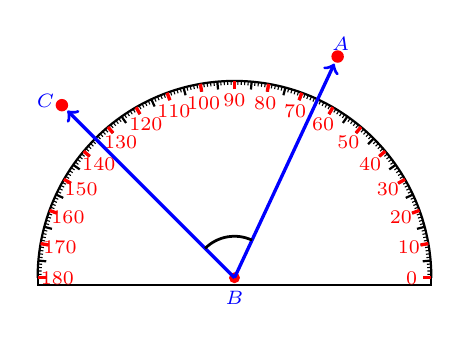
\begin{tikzpicture}[scale=0.5,font=\fontsize{7}{7}\selectfont]
\draw[thick] (5,0) arc (0:180:5);
\draw[thick] (5,0) -- (5,-5pt) -- (-5,-5pt) -- (-5,0);
%
\draw[red,fill=red] (0,0) circle (3.5pt);
% Grados
\foreach \ang in {0,1,...,180}
        \draw[rotate=\ang] (4.9,0) -- (5.0,0);
% Multiplos de 5
\foreach \mult in {0, 5,..., 180}
        \draw[thick,rotate=\mult] (4.8,0) -- (5.0,0);
% Multiplos de 10 (Solamente nodos)
\foreach \nodo in {0, 10, ...,180}
        \node[red] at (\nodo:4.5) {\nodo};
% Multiplos de 10 [los últimos]
\foreach \ult in {0, 10, ...,180}
        \draw[very thick,rotate=\ult,red]       (4.8,0) -- (5.0,0);
%\draw [help lines] (-4.5,0) grid (5,6);
\draw[blue, line width=1.2pt,rotate=65,->] (0,0) - -  (6,0);
\draw[blue, line width=1.2pt,rotate=135,->] (0,0) - -  (6,0);
\draw[color=blue] (2.7,5.95) node {$A$};
\draw[color=blue] (-4.8,4.5) node {$C$};
\draw[color=blue] (0,-0.5) node {$B$};
\fill [color=red,rotate=65] (6.2,0) circle (4.5pt);
\fill [color=red,rotate=135] (6.2,0) circle (4.5pt);
\draw[rotate=65,line width=1pt]
 (30pt,0pt) arc (0:70:30pt);
\end{tikzpicture}}{Medida de un ángulo}{meda}
 \end{figura}{Transportador}{trans}
 \end{ejemplo}
\solucion \, Usando el postulado del transportador y la definición de medida de un ángulo, de la figura(\ref{meda})
obtenemos: $\angle ABC=|135-65|=70º$
\begin{definicion}{Dos ángulos son congruentes si y sólo si tiene la misma
medida.}{Ángulos congruentes}
\end{definicion}
\begin{ejemplo}{Todos los ángulos rectos son congruentes.}
 \end{ejemplo}

\nota\,\textbf{Clasificación de los ángulos según su medida.}
\begin{lista}
 \item \textbf{Ángulo nulo:} Es un ángulo es que tiene con medida cero, es decir
sus lados coinciden.
 \item \textbf{Ángulo agudo:} Es un ángulo que tiene una medida mayor que cero y menor de 90 grados.
 \item \textbf{Ángulo recto:} Es un ángulo que tiene como medida 90 grados.
 \item \textbf{Ángulo obtuso:} Es un ángulo que tiene una medida mayor de 90 y menor de 180 grados.
 \item \textbf{Ángulo llano: } Es un ángulo que mide 180 grados, es decir sus lados forman una linea recta.
\end{lista}
\begin{figura}{\definecolor{qqwuqq}{rgb}{0,0.39,0}
\definecolor{uququq}{rgb}{0.25,0.25,0.25}
\definecolor{qqqqff}{rgb}{0,0,1}
\begin{tikzpicture}[font=\fontsize{7}{7}\selectfont,scale=0.6, line cap=round,line join=round,>=triangle 45,x=1.0cm,y=1.0cm]
\clip(-3.86,-5.96) rectangle (10.71,4.89);
\draw[color=qqwuqq,fill=qqwuqq,fill opacity=0.1] (-1.47,-2.14) -- (-1.48,-1.67) -- (-1.94,-1.67) -- (-1.94,-2.14) -- cycle;
\draw [->] (-2.06,3.1) -- (1.88,3.14);
\draw [->] (4.56,3.04) -- (8.36,3.02);
\draw [->] (4.56,3.04) -- (7.4,4.42);
\draw [->] (-1.94,-2.14) -- (-1.98,0.94);
\draw [->] (-1.94,-2.14) -- (1.64,-2.12);
\draw [->] (4.54,-2.1) -- (9,-2.12);
\draw [->] (4.54,-2.1) -- (2.86,0.78);
\draw [shift={(4.54,-2.1)}] plot[domain=0:2.1,variable=\t]({1*1.24*cos(\t r)+0*1.24*sin(\t r)},{0*1.24*cos(\t r)+1*1.24*sin(\t r)});
\draw [shift={(4.56,3.04)}] plot[domain=-0.01:0.45,variable=\t]({1*1.22*cos(\t r)+0*1.22*sin(\t r)},{0*1.22*cos(\t r)+1*1.22*sin(\t r)});
\draw [->] (2.66,-4.71) -- (-1.04,-4.73);
\draw [->] (1.18,-4.71) -- (7.03,-4.68);
\draw [shift={(2.66,-4.71)}] plot[domain=0:3.15,variable=\t]({1*1.25*cos(\t r)+0*1.25*sin(\t r)},{0*1.25*cos(\t r)+1*1.25*sin(\t r)});
\draw (-1.39,2.86) node[anchor=north west] {ángulo nulo};
\draw (5.71,2.8) node[anchor=north west] {ángulo agudo};
\draw (-1.15,-0.46) node[anchor=north west] {ángulo recto};
\draw (6.42,-1.08) node[anchor=north west] {ángulo obtuso};
\draw (4.59,-3.85) node[anchor=north west] {ángulo llano};
\fill [color=qqqqff] (-2.06,3.1) circle (1.5pt);
\draw[color=qqqqff] (-2.43,3.26) node {$A$};
\fill [color=qqqqff] (0.18,3.14) circle (1.5pt);
\draw[color=qqqqff] (0.35,3.43) node {$B$};
\fill [color=qqqqff] (4.56,3.04) circle (1.5pt);
\draw[color=qqqqff] (4.2,3.1) node {$C$};
\fill [color=qqqqff] (8.36,3.02) circle (1.5pt);
\draw[color=qqqqff] (8.53,3.3) node {$D$};
\fill [color=qqqqff] (7.4,4.42) circle (1.5pt);
\draw[color=qqqqff] (7.58,4.71) node {$E$};
\fill [color=qqqqff] (-1.96,-0.18) circle (1.5pt);
\draw[color=qqqqff] (-2.4,-0.06) node {$F$};
\fill [color=qqqqff] (-1.94,-2.14) circle (1.5pt);
\draw[color=qqqqff] (-2.32,-2.33) node {$G$};
\fill [color=uququq] (0.02,-2.12) circle (1.5pt);
\draw[color=uququq] (0.02,-2.44) node {$H$};
\fill [color=qqqqff] (4.54,-2.1) circle (1.5pt);
\draw[color=qqqqff] (4.22,-2.64) node {$K$};
\fill [color=qqqqff] (9,-2.12) circle (1.5pt);
\draw[color=qqqqff] (9.15,-1.82) node {$L$};
\fill [color=qqqqff] (2.86,0.78) circle (1.5pt);
\draw[color=qqqqff] (3.05,1.06) node {$M$};
\fill [color=qqqqff] (2.66,-4.71) circle (1.5pt);
\draw[color=qqqqff] (2.66,-5.15) node {$R$};
\fill [color=qqqqff] (-1.04,-4.73) circle (1.5pt);
\draw[color=qqqqff] (-0.86,-4.44) node {$S$};
\fill [color=qqqqff] (7.03,-4.68) circle (1.5pt);
\draw[color=qqqqff] (7.21,-4.4) node {$U$};
\end{tikzpicture}}{Clasificación de los ángulos}{claa}
 \end{figura}
\begin{definicion}{Dos rectas son perpendiculares si y sólo si
al intersectarse forman un ángulo de $90º$}{Rectas perpediculares}
 \begin{figura}{\definecolor{qqwuqq}{rgb}{0,0.39,0}
\begin{tikzpicture}[scale=0.7,font=\fontsize{7}{7}\selectfont,line cap=round,line join=round,>=triangle 45,x=1.0cm,y=1.0cm]
\clip(0.66,-1.88) rectangle (9.56,5.1);
\draw[color=qqwuqq,fill=qqwuqq,fill opacity=0.1] (3.54,0.91) -- (3.53,1.34) -- (3.11,1.32) -- (3.12,0.9) -- cycle;
\draw [domain=0.66:7.56,<->] plot(\x,{(--5.31--0.22*\x)/6.66});
\draw [domain=0.66:7.56,<->] plot(\x,{(-20.97--6.66*\x)/-0.22});
\draw (3.36,3.58) node[anchor=north west] {$l_1$};
\draw (5.86,1) node[anchor=north west] {$l_2$};
\draw[color=black] (-4.12,0.48) node {$a$};
\draw[color=black] (3.16,6.14) node {$b$};
\draw[color=qqwuqq] (4.4,1.32) node {$\alpha = 90\textrm{\degre}$};
\end{tikzpicture}}{Rectas perpendiculares}{recper}
   \end{figura}
\end{definicion}
\begin{definicion}{Una recta es perpendicular a un plano
si y sólo si la recta es perpendicular a cualquier
recta que pase por el punto de intersección de la recta y
el plano.}{Recta perpendicular a un plano}
\begin{figura}{\definecolor{qqqqff}{rgb}{0,0,1}
\definecolor{zzttqq}{rgb}{0.6,0.2,0}
\begin{tikzpicture}[scale=0.7,font=\fontsize{7}{7}\selectfont,line cap=round,line join=round,>=triangle 45,x=1.0cm,y=1.0cm]
\clip(3.21,2.01) rectangle (10.7,7.74);
\fill[color=zzttqq,fill=zzttqq,fill opacity=0.1] (3.6,5.85) -- (5.27,4.43) -- (9.84,4.35) -- (7.45,5.85) -- cycle;
\draw [color=zzttqq] (3.6,5.85)-- (5.27,4.43);
\draw [color=zzttqq] (5.27,4.43)-- (9.84,4.35);
\draw [color=zzttqq] (9.84,4.35)-- (7.45,5.85);
\draw [color=zzttqq] (7.45,5.85)-- (3.6,5.85);
\draw [->,line width=1.2pt] (5.75,5.15) -- (5.77,7.13);
\draw [->] (5.75,5.15) -- (6.67,5.65);
\draw [->] (5.75,5.15) -- (5.14,4.82);
\draw [->] (5.75,5.15) -- (6.29,4.5);
\draw [->] (5.75,5.15) -- (7.49,4.71);
\draw [->] (5.75,5.15) -- (4.51,5.46);
\draw (7.61,5.25) node[anchor=north west] {$l_1$};
\draw (6.74,5.99) node[anchor=north west] {$l_2$};
\draw (6.41,5.05) node[anchor=north west] {$r$};
\draw (8.61,5.12) node[anchor=north west] {$\xi$};
\draw (6.03,7.3) node[anchor=north west] {$l$};
\draw [->,dotted] (5.77,7.13) -- (5.75,2.51);
\fill [color=qqqqff] (5.75,5.15) circle (1.5pt);
\draw[color=qqqqff] (5.96,5.59) node {$E$};
\end{tikzpicture}}{Recta perpendicular a un plano}{recpp}
 \end{figura}
\end{definicion}
\begin{definicion}{Dos planos son perpendicularessi en uno de ellos
hay una recta perpendicular al otro.}{Planos perpendiculares}
\begin{figura}{\definecolor{xdxdff}{rgb}{0.49,0.49,1}
\definecolor{zzttqq}{rgb}{0.6,0.2,0}
\begin{tikzpicture}[scale=0.7,font=\fontsize{7}{7}\selectfont,line cap=round,line join=round,>=triangle 45,x=1.0cm,y=1.0cm]
\clip(-0.5,2.7) rectangle (6.62,8.34);
\fill[color=zzttqq,fill=zzttqq,fill opacity=0.1] (1.88,3.58) -- (4.72,5.76) -- (4.7,7.88) -- (1.8,5.74) -- cycle;
\fill[color=zzttqq,fill=zzttqq,fill opacity=0.1] (5.88,6.6) -- (5.9,4.3) -- (-0.06,4.26) -- (-0.04,6.5) -- cycle;
\fill[color=zzttqq,fill=zzttqq,fill opacity=0.1] (2.83,5.42) -- (3.16,5.42) -- (3.45,5.62) -- (3.13,5.61) -- cycle;
\draw [color=zzttqq] (1.88,3.58)-- (4.72,5.76);
\draw [color=zzttqq] (4.72,5.76)-- (4.7,7.88);
\draw [color=zzttqq] (4.7,7.88)-- (1.8,5.74);
\draw [color=zzttqq] (1.8,5.74)-- (1.88,3.58);
\draw [color=zzttqq] (5.88,6.6)-- (5.9,4.3);
\draw [color=zzttqq] (5.9,4.3)-- (-0.06,4.26);
\draw [color=zzttqq] (-0.06,4.26)-- (-0.04,6.5);
\draw [color=zzttqq] (-0.04,6.5)-- (5.88,6.6);
\draw (2.87,6.53)-- (2.8,4.28);
\draw [->] (2.83,5.42) -- (4.46,6.46);
\draw [->] (2.83,5.42) -- (5.48,5.42);
\draw [color=zzttqq] (2.83,5.42)-- (3.16,5.42);
\draw [color=zzttqq] (3.16,5.42)-- (3.45,5.62);
\draw [color=zzttqq] (3.45,5.62)-- (3.13,5.61);
\draw [color=zzttqq] (3.13,5.61)-- (2.83,5.42);
\draw (0.18,5) node[anchor=north west] {$\xi$};
\draw (5.5,4.98) node[anchor=north west] {$\pi$};
\fill [color=xdxdff] (2.87,6.53) circle (1.5pt);
\draw[color=xdxdff] (2.74,6.8) node {$I$};
\fill [color=xdxdff] (2.8,4.28) circle (1.5pt);
\draw[color=xdxdff] (2.72,3.98) node {$J$};
\fill [color=xdxdff] (2.83,5.42) circle (1.5pt);
\end{tikzpicture}}{Planos perpendiculares}{pperp}
\end{figura}
\end{definicion}
\seccion{Construcciones básicas}
\label{sec:1.4}
\hskip -20pt
\begin{floatingfigure}[lrp]{4cm}

 %\begin{center}
 \centering
 \includegraphics[scale=0.3]{./herramientas.jpg}
%\end{center}
\end{floatingfigure}
Los diseñadores utilizan una variedad de instrumentos y técnicas para
ela\-borar sus diseños, a los cuales no se les puede aprovechar en su totalidad,
si no se conocen y se aplican las propiedades de los elementos  y los conceptos
de la geometría.
\vskip 20pt
En esta sección presentaremos las construcciones de las cuales se basan la
mayoría
 de las construcciones más complicadas que utilizaremos en el libro.
\begin{construccion}{Para duplicar un segmento hay que realizar los siguientes pasos
\begin{lista}
 \item Se construye un segmento.
 \item  Se colocan las puntas de un compás en los extremos del segmento.
 \item se construye un rayo o una recta donde queremos duplicar el segmento
 \item Se coloca la punta filosa del compás en un punto de la recta, manteniendo la abertura del primer
  paso y se dibuja  con la otra punta un peque\~no. arco sobre la recta.
  \item El punto de intersección de la recta y el arco es el otro extremo del segmento.
\end{lista}
}{Duplicar un segmento}
\end{construccion}

 \begin{figura}{
 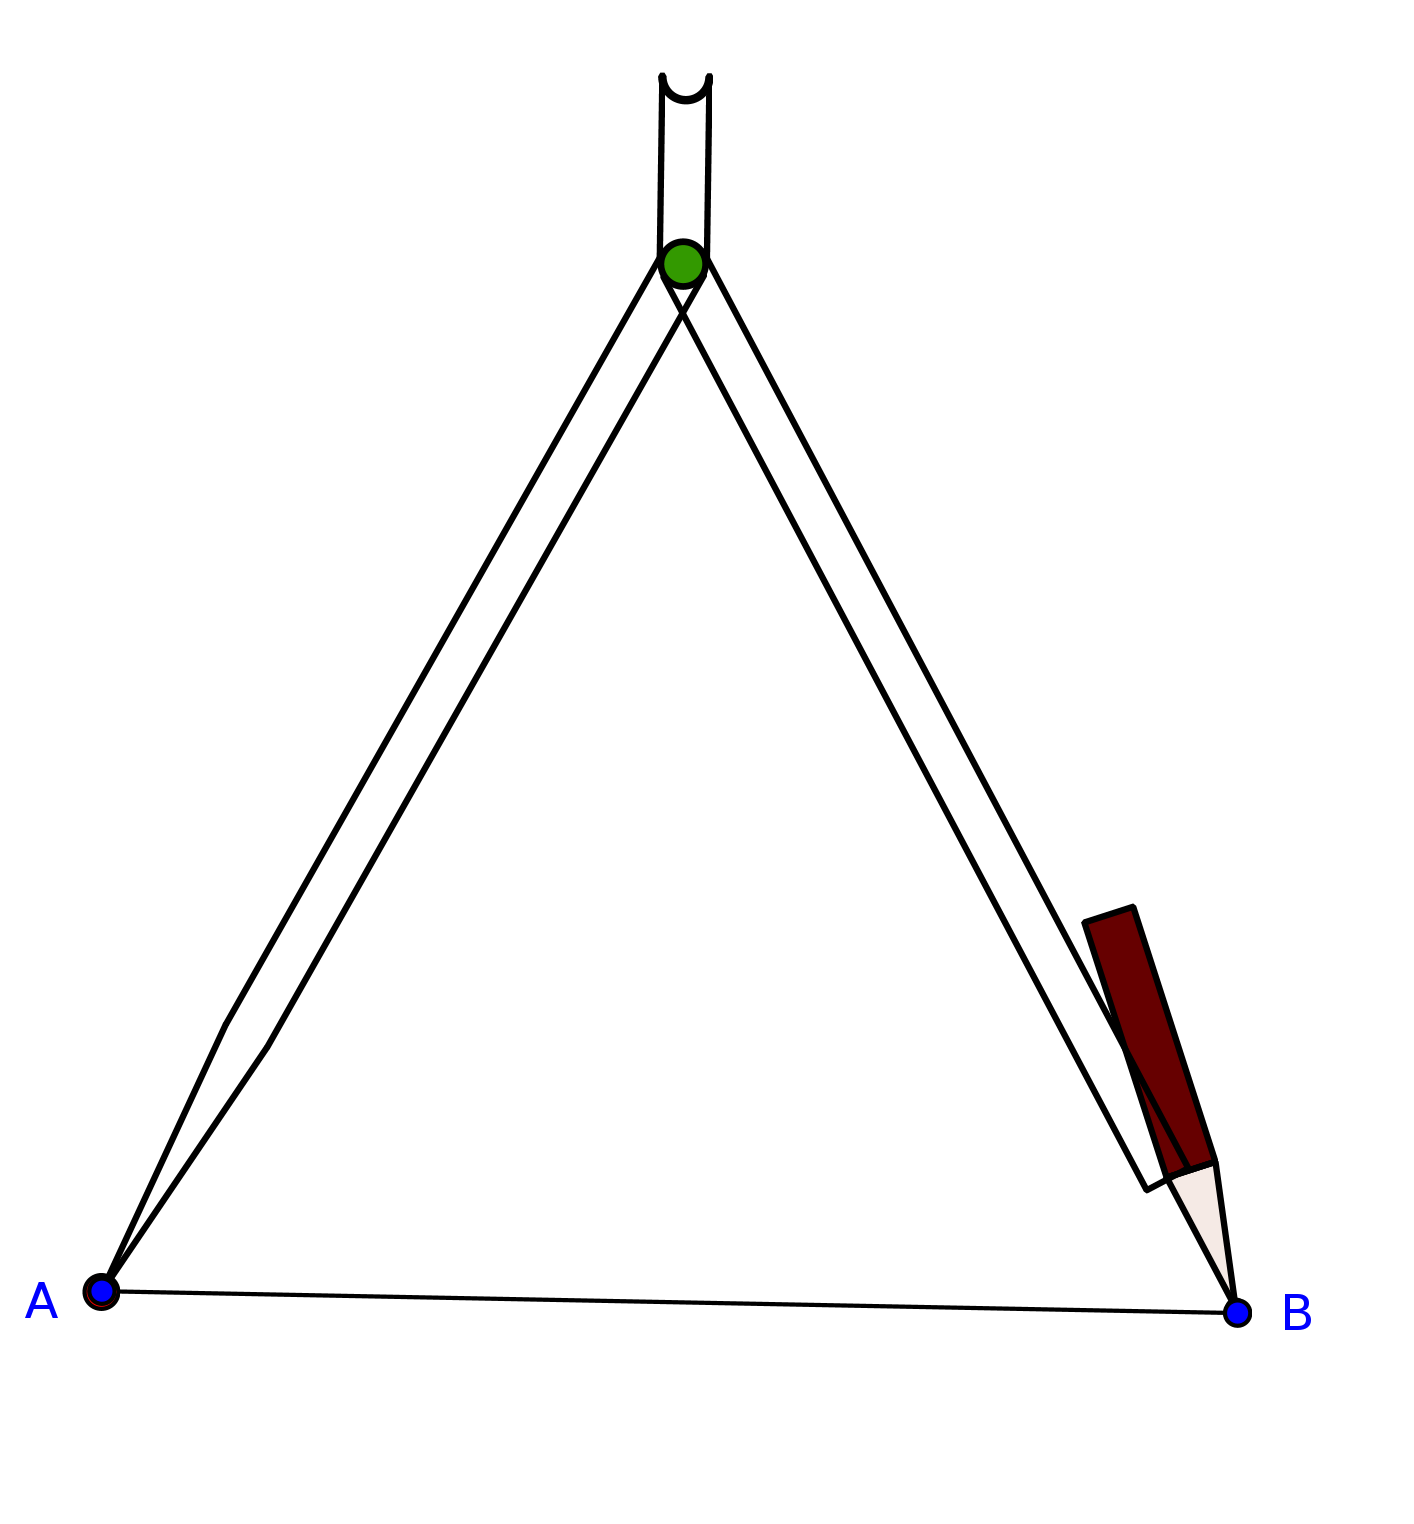
\includegraphics[scale=0.4]{./compas1.png}
 % compas1.png: 1414x1524 pixel, 300dpi, 11.97x12.90 cm, bb=0 0 339 366
}{Segmento dado}{segd}
 \end{figura}
\hfill
 \begin{figura}{
 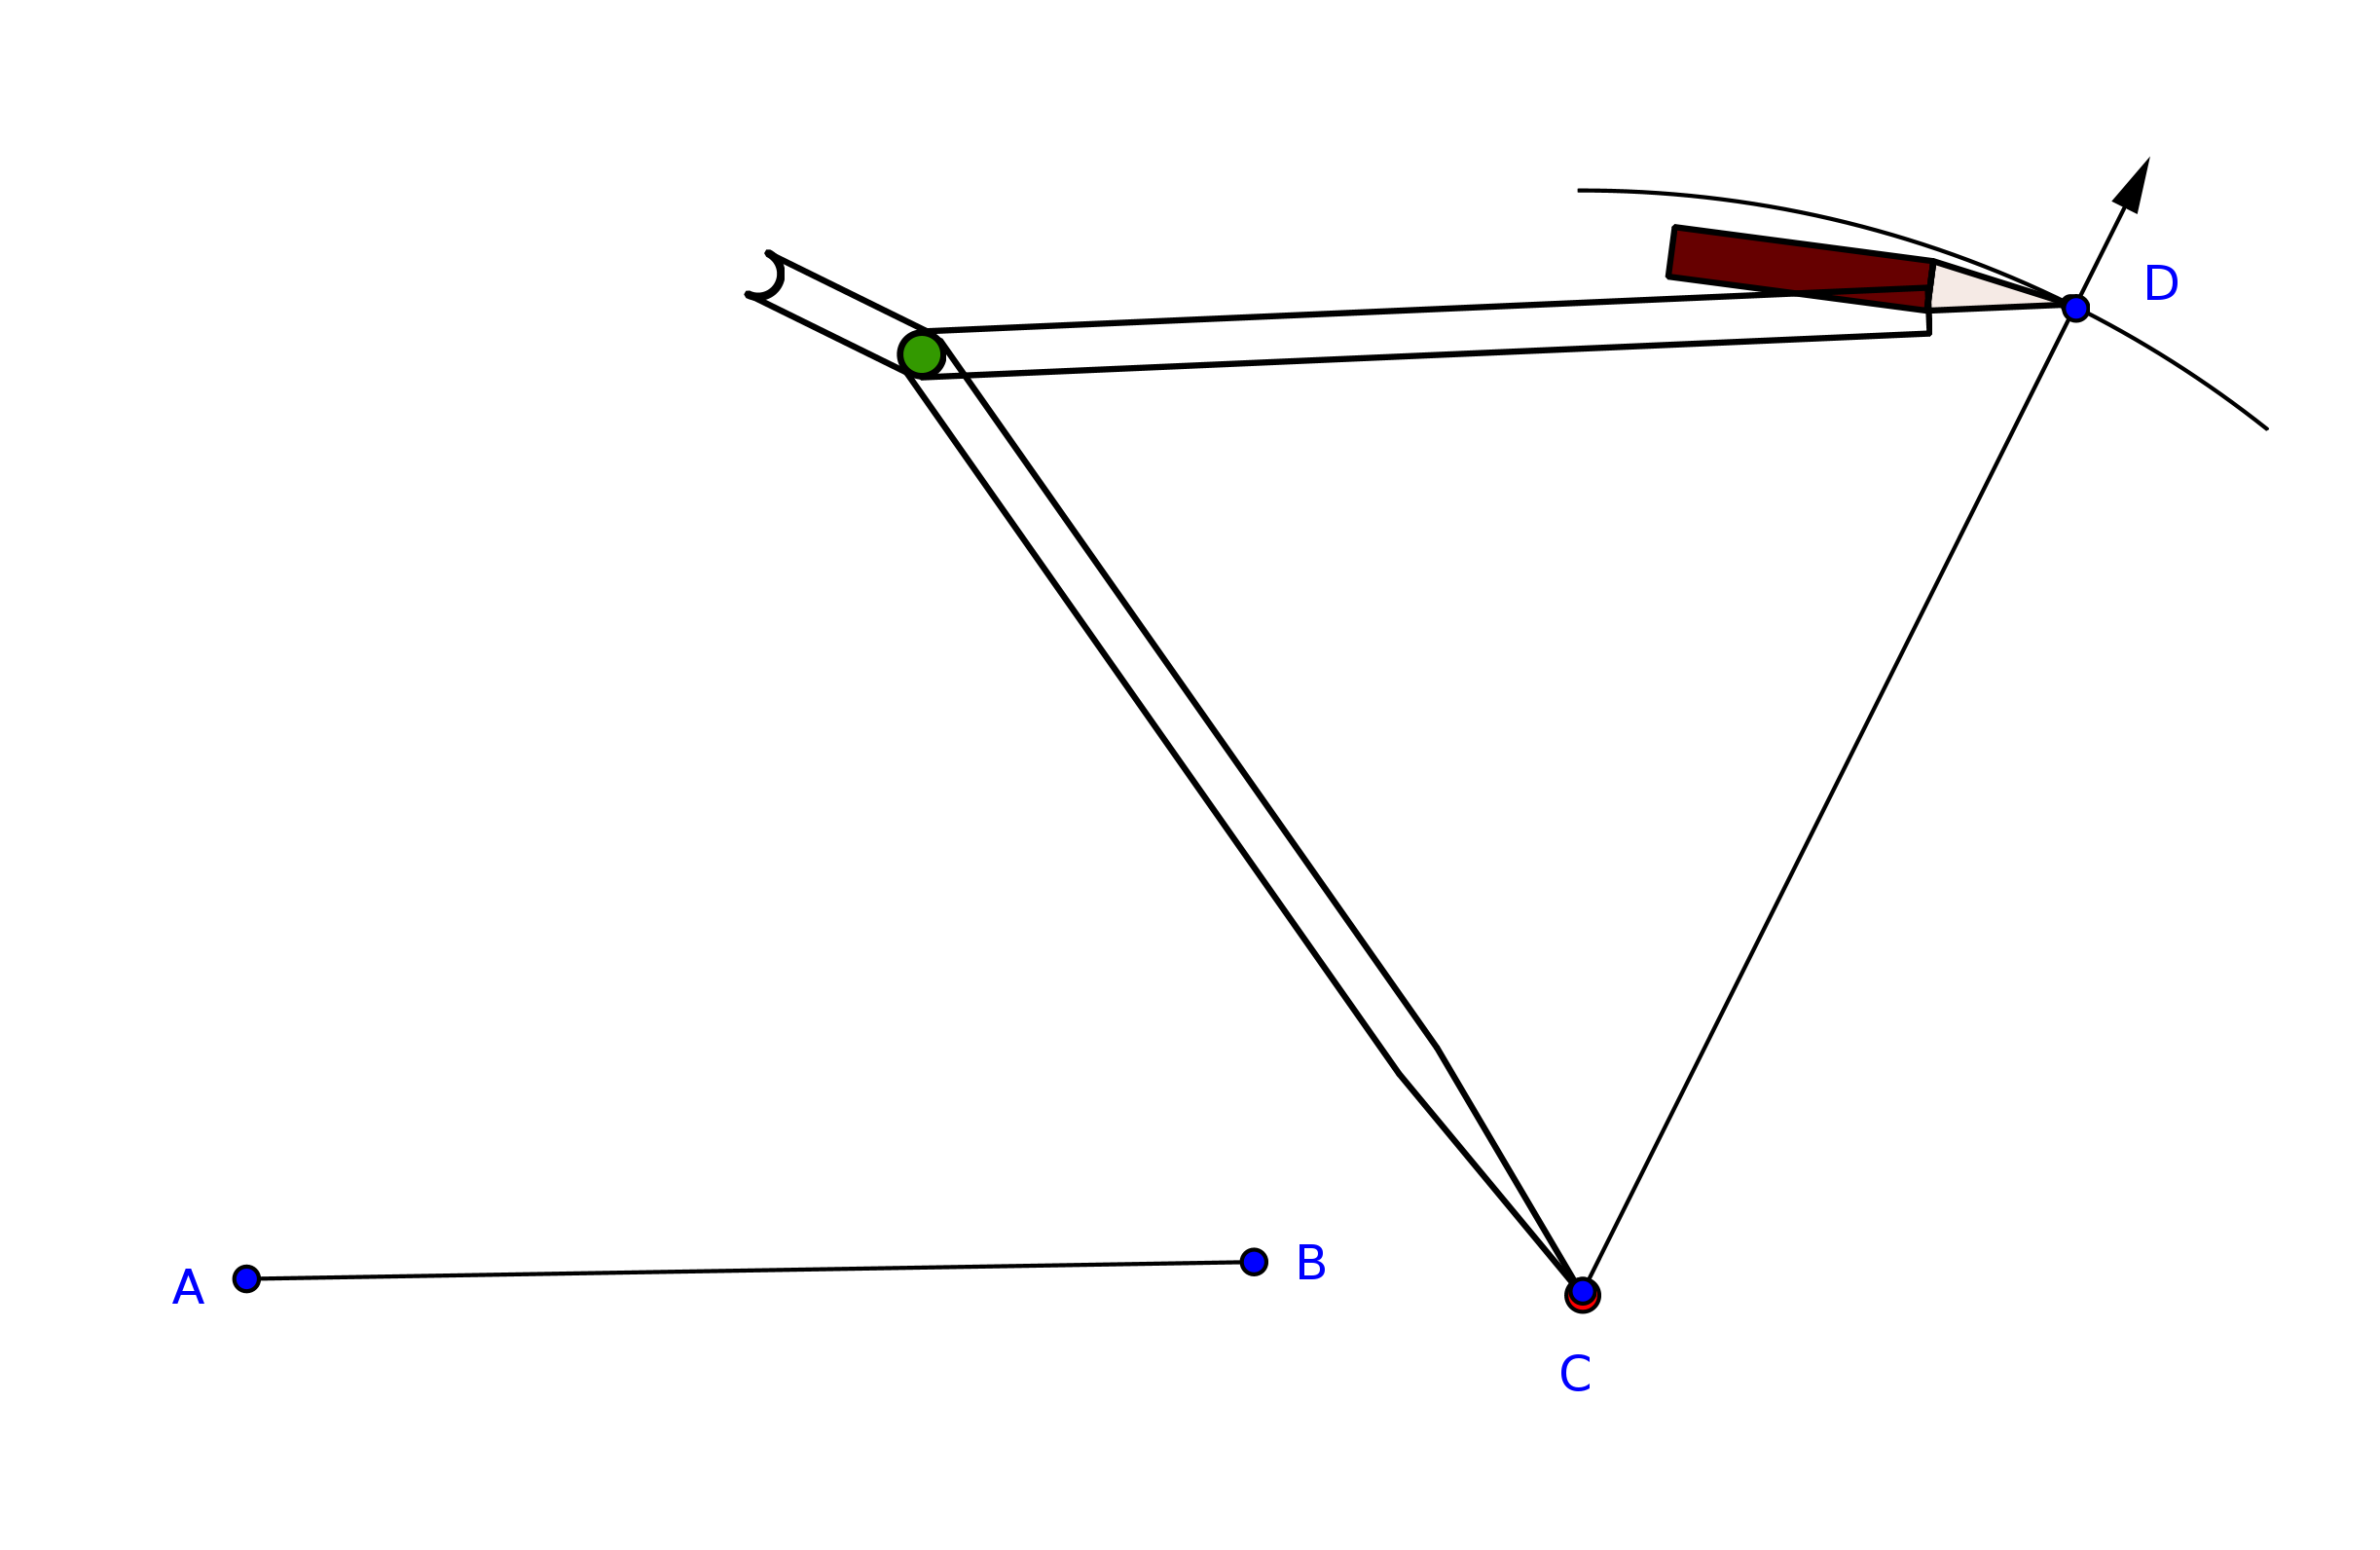
\includegraphics[scale=0.4]{./compas2.png}
 % compas1.png: 1414x1524 pixel, 300dpi, 11.97x12.90 cm, bb=0 0 339 366
}{Segmento duplicado}{segdp}
\end{figura}
De acuerdo con la construcción los segmentos $AB$ y $CD$ de la figura(\ref{segdp})
son congruentes.
\begin{ejemplo}{Un triángulo es un polígono de tres lados, usando esta definición. Construya
Un triángulo con dos lados congruentes.}
 \end{ejemplo}
\solucion En el triángulo de la figura(\ref{trii}) los lados $AB$ y $AC$ son congruentes.
\begin{figura}{
\definecolor{qqqqff}{rgb}{0,0,1}
\begin{tikzpicture}[font=\fontsize{7}{7}\selectfont,scale=1.9,line cap=round,line join=round,>=triangle 45,x=1.0cm,y=1.0cm]
\clip(2.21,0.88) rectangle (6.59,4.32);
\draw [line width=1.2pt,->] (2.98,2.28) -- (5.17,3.6);
\draw [line width=1.2pt,->] (2.98,2.28) -- (6.07,1.49);
\draw [line width=1.2pt,shift={(2.98,2.28)}] plot[domain=-0.74:0.85,variable=\t]({1*1.64*cos(\t r)+0*1.64*sin(\t r)},{0*1.64*cos(\t r)+1*1.64*sin(\t r)});
\draw (2.98,2.28)-- (4.57,1.87);
\draw (3.62,3) node[anchor=north west] {a};
\draw [line width=1.2pt](4.57,1.87)-- (4.39,3.13);
\fill [color=qqqqff] (2.98,2.28) circle (2.0pt);
\draw[color=qqqqff] (2.88,2.28) node {$A$};
\fill [color=qqqqff] (4.57,1.87) circle (1.5pt);
\draw[color=qqqqff] (4.66,1.75) node {$B$};
\fill [color=qqqqff] (4.39,3.13) circle (1.5pt);
\draw[color=qqqqff] (4.41,3.31) node {$C$};
\draw[color=black] (3.77,2) node {$a$};
\draw[color=black] (4.37,2.51) node {$b$};
\end{tikzpicture}}{Triángulo isósceles.}{trii}
\end{figura}

\begin{construccion}{
Para construir dos ángulos congruentes se realizan los siguientes pasos:
\begin{lista}
 \item Dado un ángulo.
\item Se traza un arco con centro en el vértice que corte a los otros dos lados,
y se marcan los puntos de intersección.
\item Se construye un rayo, para que sea un lado del ángulo a duplicado.
\item Con la misma abertura del compás se traza un arco sobre el rayo, con centro
en el origen del rayo.
\item Coloque la puntas del compás sobre los puntos de intersección del arco y los lados del ángulo dado.
\item En el punto de intersección del arco y el rayo trace un nuevo arco centrado en este punto
 y con la misma abertura del compás del paso anterior.
\item una el punto de interseccion de los arcos trazados sobre el rayo y el
origen de este.
\end{lista}
}{Ángulos congruentes}
\begin{figura}{
\definecolor{xdxdff}{rgb}{0.49,0.49,1}
\definecolor{qqqqff}{rgb}{0,0,1}
\begin{tikzpicture}[font=\fontsize{7}{7}\selectfont,scale=1.9,line cap=round,line join=round,>=triangle 45,x=1.0cm,y=1.0cm]
\clip(2.28,0.61) rectangle (11.05,4.48);
\draw [line width=1.2pt,->] (2.98,2.28) -- (5.17,3.6);
\draw [line width=1.2pt,->] (2.98,2.28) -- (6.07,1.49);
\draw [line width=1.2pt,->] (7.13,1.33) -- (10.63,1.32);
\draw [line width=1.2pt,shift={(2.98,2.28)}] plot[domain=-0.74:0.85,variable=\t]({1*1.64*cos(\t r)+0*1.64*sin(\t r)},{0*1.64*cos(\t r)+1*1.64*sin(\t r)});
\draw [line width=1.2pt](2.98,2.28)-- (4.57,1.87);
\draw [line width=1.2pt,shift={(7.13,1.33)}] plot[domain=0:1.28,variable=\t]({1*1.64*cos(\t r)+0*1.64*sin(\t r)},{0*1.64*cos(\t r)+1*1.64*sin(\t r)});
\draw (7.8,1.29) node[anchor=north west] {a};
\draw [line width=1.2pt] (4.57,1.87)-- (4.39,3.13);
\draw [line width=1.2pt,shift={(8.77,1.33)}] plot[domain=1.96:3.43,variable=\t]({1*1.26*cos(\t r)+0*1.26*sin(\t r)},{0*1.26*cos(\t r)+1*1.26*sin(\t r)});
\draw [line width=1.2pt](8.77,1.33)-- (8.28,2.49);
\draw (8.36,2) node[anchor=north west] {b};
\draw [line width=1.2pt,shift={(8.77,1.33)}] plot[domain=1.63:3.25,variable=\t]({1*1.27*cos(\t r)+0*1.27*sin(\t r)},{0*1.27*cos(\t r)+1*1.27*sin(\t r)});
\draw [line width=1.2pt,line width=1.2pt,->] (7.13,1.33) -- (9.03,3.24);
\fill [color=qqqqff] (2.98,2.28) circle (1.5pt);
\draw[color=qqqqff] (2.78,2.28) node {$A$};
\fill [color=qqqqff] (4.57,1.87) circle (1.5pt);
\draw[color=qqqqff] (4.66,1.75) node {$B$};
\fill [color=qqqqff] (4.39,3.13) circle (1.5pt);
\draw[color=qqqqff] (4.41,3.31) node {$C$};
\fill [color=qqqqff] (7.13,1.33) circle (1.5pt);
\draw[color=qqqqff] (7.02,1.38) node {$D$};
\draw[color=black] (3.77,2) node {$a$};
\fill [color=xdxdff] (8.77,1.33) circle (1.5pt);
\draw[color=xdxdff] (8.83,1.2) node {$E$};
\draw[color=black] (4.37,2.51) node {$b$};
\fill [color=xdxdff] (8.28,2.49) circle (1.5pt);
\draw[color=xdxdff] (8.24,2.34) node {$F$};
\end{tikzpicture}}{Ángulos congruentes}{angc}
 \end{figura}
\end{construccion}
\begin{ejemplo}{Construya un triángulo con dos ángulos congruentes. }
\begin{figura}{
\definecolor{xdxdff}{rgb}{0.49,0.49,1}
\definecolor{qqqqff}{rgb}{0,0,1}
\begin{tikzpicture}[font=\fontsize{8}{8}\selectfont,scale=3.0,line cap=round,line join=round,>=triangle 45,x=1.0cm,y=1.0cm]
\clip(1.34,-0.23) rectangle (4.12,1.92);
\draw [line width=1.2pt,->] (1.61,0.24) -- (2.79,1.76);
\draw [line width=1.2pt,->] (1.61,0.24) -- (4.04,0.24);
\draw [line width=1.2pt,shift={(1.61,0.24)}] plot[domain=0:1.23,variable=\t]({1*0.82*cos(\t r)+0*0.82*sin(\t r)},{0*0.82*cos(\t r)+1*0.82*sin(\t r)});
\draw [line width=1.2pt](1.61,0.24)-- (2.43,0.24);
\draw [line width=1.2pt,shift={(3.66,0.24)}] plot[domain=1.9:3.14,variable=\t]({1*0.82*cos(\t r)+0*0.82*sin(\t r)},{0*0.82*cos(\t r)+1*0.82*sin(\t r)});
\draw [line width=1.2pt](2.43,0.24)-- (2.11,0.89);
\draw [line width=1.2pt,shift={(2.43,0.24)}] plot[domain=2.03:2.39,variable=\t]({1*0.72*cos(\t r)+0*0.72*sin(\t r)},{0*0.72*cos(\t r)+1*0.72*sin(\t r)});
\draw [line width=1.2pt,shift={(2.43,0.24)}] plot[domain=1.77:2.5,variable=\t]({1*0.73*cos(\t r)+0*0.73*sin(\t r)},{0*0.73*cos(\t r)+1*0.73*sin(\t r)});
\draw [line width=1.2pt,shift={(2.83,0.23)}] plot[domain=0.01:1.39,variable=\t]({1*0.71*cos(\t r)+0*0.71*sin(\t r)},{0*0.71*cos(\t r)+1*0.71*sin(\t r)});
\draw [line width=1.2pt](3.66,0.24)-- (2.49,1.74);
\draw [line width=1.2pt,->] (3.66,0.24) -- (2.57,0.24);
\draw [line width=1.2pt,->] (2.81,1.34) -- (2.47,1.77);
\fill [color=qqqqff] (1.61,0.24) circle (1.0pt);
\draw[color=qqqqff] (1.48,0.24) node {$A$};
\fill [color=xdxdff] (2.43,0.24) circle (1.0pt);
\draw[color=xdxdff] (2.44,0.16) node {$B$};
\fill [color=xdxdff] (3.66,0.24) circle (1.0pt);
\draw[color=xdxdff] (3.67,0.17) node {$D$};
\fill [color=qqqqff] (2.11,0.89) circle (1.0pt);
\draw[color=qqqqff] (2.1,1.03) node {$C$};
\draw[color=black] (2.04,0.19) node {$a$};
\draw[color=black] (2.19,0.54) node {$b$};
\fill [color=qqqqff] (2.83,0.23) circle (1.0pt);
\draw[color=qqqqff] (2.83,0.14) node {$E$};
\fill [color=qqqqff] (3.15,0.88) circle (1.0pt);
\draw[color=qqqqff] (3.17,1.02) node {$F$};
\fill [color=qqqqff] (2.63,1.56) circle (1.0pt);
\draw[color=qqqqff] (2.62,1.71) node {$G$};
\end{tikzpicture}}{Triángulo con dos ángulos congruentes}{triaa}
 \end{figura}
En el \triangulo $ADG$ los ángulos $ABC$ y $EDF$ son congruentes.
\end{ejemplo}



\begin{construccion}{Para bisecar un ángulo se realizan los siguientes
pasos:
\begin{lista}
 \item Dado un segmento
\item Se traza una semi circunferencia con centro en un extremo
del segmento y que lo intersecte en un punto.
\item Se traza una semi circunferencia con centro en el otro extremo, de tal
forma que intersecte al primero.
\item Se traza un segmento con extremos en los puntos de intersección de las semi circunferencias.
\item El punto de intersección de los dos segmentos es el punto medio.
\end{lista}
}{Punto medio de un segmento}
\begin{figura}{\definecolor{uququq}{rgb}{0.25,0.25,0.25}
\definecolor{qqqqff}{rgb}{0,0,1}
\begin{tikzpicture}[font=\fontsize{7}{7}\selectfont,scale=0.3,line cap=round,line join=round,>=triangle 45,x=1.0cm,y=1.0cm]
\clip(-17.82,-11.18) rectangle (19.74,13.88);
\draw [line width=1.2pt] (-5.03,2.12)-- (4.09,2.12);
\draw(-5.03,2.12) circle (9.12cm);
\draw(4.09,2.12) circle (9.11cm);
\draw [line width=1.2pt,dash pattern=on 5pt off 5pt] (-0.46,10.01)-- (-0.46,-5.78);
\draw [->] (3.92,-2.83) -- (-0.46,2.12);
\draw (3.16,-2.86) node[anchor=north west] {Punto medio};
\fill [color=qqqqff] (-5.03,2.12) circle (1.5pt);
\draw[color=qqqqff] (-6.69,2.37) node {$A$};
\fill [color=qqqqff] (4.09,2.12) circle (1.5pt);
\draw[color=qqqqff] (5.28,2.52) node {$B$};
\fill [color=uququq] (-0.46,10.01) circle (1.5pt);
\draw[color=uququq] (-0.63,12.21) node {$D$};
\fill [color=uququq] (-0.46,-5.78) circle (1.5pt);
\draw[color=uququq] (-0.63,-7.7) node {$E$};
\fill [color=uququq] (-0.46,2.12) circle (1.5pt);
\draw[color=uququq] (0.05,3.13) node {$F$};
\end{tikzpicture}}{Punto medio}{pm}
 \end{figura}
\end{construccion}
\begin{definicion}{La bisectriz de de un segmento
es una recta que pasa por el punto medio del segmento. }{Bisectriz de un
segmento}
\end{definicion}
\begin{construccion}{Para construir la bisectriz de un segmento que pasa por un punto
 no alineado con el segmento, se realizan los siguientes pasos.
\begin{lista}
 \item Dado un segmento y un punto no alineado.
 \item Se construye el punto medio del segmento.
 \item la bisectriz es la recta que pasa por el punto no alineado y el puto medio.
\end{lista}
}{Bisectriz de un segmento}
\begin{figura}{
\definecolor{uququq}{rgb}{0.25,0.25,0.25}
\definecolor{qqqqff}{rgb}{0,0,1}
\begin{tikzpicture}[font=\fontsize{7}{7}\selectfont,scale=2.8,line cap=round,line join=round,>=triangle 45,x=1.0cm,y=1.0cm]
\clip(0.47,-1.25) rectangle (3.45,1.12);
\draw [line width=1.2pt](1.68,-0.07)-- (2.66,-0.06);
\draw [line width=1.2pt,shift={(2.66,-0.06)}] plot[domain=3.16:4.97,variable=\t]({1*0.98*cos(\t r)+0*0.98*sin(\t r)},{0*0.98*cos(\t r)+1*0.98*sin(\t r)});
\draw [line width=1.2pt,shift={(1.68,-0.07)}] plot[domain=0.02:1.87,variable=\t]({1*0.98*cos(\t r)+0*0.98*sin(\t r)},{0*0.98*cos(\t r)+1*0.98*sin(\t r)});
\draw [line width=1.2pt,shift={(1.68,-0.07)}] plot[domain=0.02:1.87,variable=\t]({1*0.98*cos(\t r)+0.03*0.98*sin(\t r)},{0.03*0.98*cos(\t r)+-1*0.98*sin(\t r)});
\draw [line width=1.2pt,shift={(2.66,-0.06)}] plot[domain=3.16:4.97,variable=\t]({1*0.98*cos(\t r)+0.03*0.98*sin(\t r)},{0.03*0.98*cos(\t r)+-1*0.98*sin(\t r)});
\draw [line width=1.2pt,dotted] (2.16,0.78)-- (2.19,-0.92);
\draw [line width=1.2pt,->](1.11,0.7)-- (3.17,-0.79);
\draw [line width=1.2pt,->](2.17,-0.07)-- (0.75,0.96);
\fill [color=qqqqff] (1.68,-0.07) circle (1.5pt);
\draw[color=qqqqff] (1.48,-0.06) node {$A$};
\fill [color=qqqqff] (2.66,-0.06) circle (1.5pt);
\draw[color=qqqqff] (2.8,-0.01) node {$B$};
\fill [color=uququq] (2.16,0.78) circle (1.5pt);
\draw[color=uququq] (2.38,0.8) node {$C$};
\fill [color=uququq] (2.19,-0.92) circle (1.5pt);
\draw[color=uququq] (1.9,-0.83) node {$D$};
\fill [color=qqqqff] (1.11,0.7) circle (1.5pt);
\draw[color=qqqqff] (1.18,0.82) node {$P$};
\fill [color=uququq] (2.17,-0.07) circle (1.5pt);
\draw[color=uququq] (2.25,0.06) node {$E$};
%\draw[color=black] (2.09,-0.1) node {$e$};
\end{tikzpicture}}{Bisectriz de un segmento}{bisecseg}
\end{figura}

\end{construccion}
\begin{definicion}{La bisectriz de un ángulo es la recta que pasa por el vértice
de un ángulo y forma dos ángulos congruentes}{Bisectriz de un ángulo}
 \end{definicion}
\begin{construccion}{Para bisecar un ángulo se realiza el siguiente
procedimiento:
\begin{lista}
 \item dado un ángulo.
 \item Se traza un arco con centro en el vértice del ángulo que corte los lados
del ángulo.
 \item En cada punto de intersección se construyen dos arcos de igual radio.
 \item Se determina el punto de intersección de los arcos.
 \item La bisectriz es la recta que pasa por el punto de corte de los arcos y el vértice
del ángulo.
\end{lista}
 }{Bisectriz de un ángulo}
\begin{figura}{\definecolor{uququq}{rgb}{0.25,0.25,0.25}
\definecolor{xdxdff}{rgb}{0.49,0.49,1}
\definecolor{qqqqff}{rgb}{0,0,1}
\begin{tikzpicture}[font=\fontsize{7}{7}\selectfont,scale=0.3, line cap=round,line join=round,>=triangle 45,x=1.0cm,y=1.0cm]
\clip(-16.07,-12.85) rectangle (12.77,12.89);
\draw [line width=1.2pt](-10.55,-2.33)-- (3.23,9.71);
\draw [line width=1.2pt](-10.55,-2.33)-- (8.23,-3.99);
\draw [line width=1.2pt,shift={(-10.55,-2.33)},line width=1.2pt,dash pattern=on 5pt off 5pt]  plot[domain=-0.09:0.72,variable=\t]({1*10.94*cos(\t r)+0*10.94*sin(\t r)},{0*10.94*cos(\t r)+1*10.94*sin(\t r)});
\draw [line width=1.2pt](0.35,-3.29) circle (6.09cm);
\draw [line width=1.2pt](0.35,-3.29)-- (-5.71,-2.75);
\draw [line width=1.2pt](-2.42,4.77) circle (6.09cm);
\draw [line width=1.2pt,->] (-10.55,-2.33) -- (3.23,9.71);
\draw [line width=1.2pt,->] (-10.55,-2.33) -- (8.23,-3.99);
\draw [line width=1.2pt,->] (0.35,-3.29) -- (-5.71,-2.75);
\draw (-2.3,-3.31) node[anchor=north west] {r};
\draw (-5.17,5.7) node[anchor=north west] {r};
\draw [line width=1.2pt,->] (-2.42,4.77) -- (-8.05,7.08);
\draw [line width=1.2pt,domain=-16.07:12.77] plot(\x,{(--15.55--4.48*\x)/13.62});
\fill [color=qqqqff] (-10.55,-2.33) circle (1.5pt);
\draw[color=qqqqff] (-11.83,-1.34) node {$A$};
\fill [color=qqqqff] (3.23,9.71) circle (1.5pt);
\draw[color=qqqqff] (3.84,10.7) node {$B$};
\fill [color=qqqqff] (8.23,-3.99) circle (1.5pt);
\draw[color=qqqqff] (8.83,-3.01) node {$D$};
\fill [color=xdxdff] (0.35,-3.29) circle (1.5pt);
\draw[color=xdxdff] (0.35,-4.29) node {$E$};
\fill [color=xdxdff] (-2.42,4.77) circle (1.5pt);
\draw[color=xdxdff] (-2.37,6.08) node {$F$};
\fill [color=xdxdff] (-5.71,-2.75) circle (1.5pt);
\draw[color=xdxdff] (-6.76,-3.92) node {$H$};
\fill [color=xdxdff] (-8.05,7.08) circle (1.5pt);
\fill [color=uququq] (3.07,2.15) circle (1.5pt);
\draw[color=uququq] (4.37,3.88) node {$J$};
\fill [color=uququq] (-5.14,-0.67) circle (1.5pt);
\draw[color=uququq] (-5.4,0.93) node {$K$};
%\draw[color=black] (-26.37,-6.34) node {$g$};
\end{tikzpicture}}{Bisectriz del ángulo}{biseca}
\end{figura}
\end{construccion}
\begin{ejemplo}{Construya una flor de 4 pétalos bisecando en ángulo  de 90 grados para cada
pétalo.}
\solucion
\begin{figura}{
\definecolor{qqqqff}{rgb}{0,0,1}
\definecolor{uququq}{rgb}{0.25,0.25,0.25}
\definecolor{ttttff}{rgb}{0.2,0.2,1}
\definecolor{ffttzz}{rgb}{1,0.2,0.6}
\begin{tikzpicture}[font=\fontsize{7}{7}\selectfont,scale=3.0,line cap=round,line join=round,>=triangle 45,x=1.0cm,y=1.0cm]
\clip(-0.09,-0.43) rectangle (3.88,2.26);
\draw (0.64,0.9) node[anchor=north west] {$l_1$};
\draw [line width=1.2pt,dotted] (0.49,0.88)-- (3.47,0.86);
\draw [line width=1.2pt,dash pattern=on 1pt off 1pton 2pt off 4pt,color=ttttff,fill=ttttff,fill opacity=0.15] (1.96,0.85) circle (0.57cm);
\draw [line width=1.2pt,dash pattern=on 1pt off 1pt on 2pt off 4pt,color=ffttzz,fill=ffttzz,fill opacity=0.05] (1.39,0.87) circle (1.14cm);
\draw [line width=1.2pt,dash pattern=on 1pt off 1pt on 2pt off 4pt,color=ffttzz,fill=ffttzz,fill opacity=0.05] (2.53,0.86) circle (1.14cm);
\draw [line width=1.2pt,dotted] (1.97,1.86)-- (1.95,-0.12);
\draw [line width=1.2pt,shift={(1.39,0.87)}] plot[domain=-1.58:1.56,variable=\t]({1*0.57*cos(\t r)+0*0.57*sin(\t r)},{0*0.57*cos(\t r)+1*0.57*sin(\t r)});
\draw [line width=1.2pt,shift={(1.96,0.3)}] plot[domain=-0.01:3.13,variable=\t]({1*0.57*cos(\t r)+0*0.57*sin(\t r)},{0*0.57*cos(\t r)+1*0.57*sin(\t r)});
\draw [line width=1.2pt,shift={(1.96,1.44)}] plot[domain=3.13:6.28,variable=\t]({1*0.57*cos(\t r)+0*0.57*sin(\t r)},{0*0.57*cos(\t r)+1*0.57*sin(\t r)});
\draw [line width=1.2pt,shift={(2.53,0.86)}] plot[domain=1.56:4.7,variable=\t]({1*0.57*cos(\t r)+0*0.57*sin(\t r)},{0*0.57*cos(\t r)+1*0.57*sin(\t r)});
\fill [color=ffttzz] (2.53,0.86) circle (1.0pt);
\draw[color=ffttzz] (2.59,0.96) node {$B$};
\fill [color=ffttzz] (1.39,0.87) circle (1.0pt);
\draw[color=ffttzz] (1.32,0.79) node {$C$};
\fill [color=uququq] (1.97,1.86) circle (1.0pt);
\draw[color=uququq] (2.09,1.88) node {$F$};
\fill [color=uququq] (1.95,-0.12) circle (1.0pt);
\draw[color=uququq] (1.79,-0.09) node {$G$};
\fill [color=uququq] (1.96,1.42) circle (1.0pt);
\draw[color=uququq] (2.03,1.51) node {$H$};
\fill [color=uququq] (1.95,0.28) circle (1.0pt);
\draw[color=uququq] (1.99,0.38) node {$I$};
\fill [color=uququq] (1.39,1.44) circle (1.0pt);
\fill [color=uququq] (2.53,1.44) circle (1.0pt);
\fill [color=uququq] (2.53,0.29) circle (1.0pt);
\fill [color=uququq] (1.38,0.3) circle (1.0pt);
\fill [color=qqqqff] (1.96,0.87) circle (1.0pt);
\draw[color=qqqqff] (2.02,0.97) node {$P$};
\end{tikzpicture}}{Flor de cuatro pétalos.}{f4pet}
\end{figura}

\end{ejemplo}

\begin{construccion}{Dado un punto de una recta.
Para construir construir una recta perpendicular que pase por el punto dados
 se realiza lo siguiente:
\begin{lista}
 \item Dado un punto en una recta.
 \item Trace un arco centrado en el punto dado que corte a la recta
en dos puntos.
 \item Trace dos arcos centrados en cada uno de los puntos de corte del paso
anterior.
 \item Trace la linea perpendicular entre el punto de intersección de los
arcos construidos en el paso anterior y el punto dado.
\end{lista}
}{Recta perpendicular dado un punto en ella}
 \end{construccion}
 \begin{figura}{
\definecolor{qqqqff}{rgb}{0,0,1}
\definecolor{xdxdff}{rgb}{0.49,0.49,1}
\begin{tikzpicture}[font=\fontsize{8}{8}\selectfont,scale=1.3, line cap=round,line join=round,>=triangle 45,x=1.0cm,y=1.0cm]
\clip(0.25,0.58) rectangle (5.98,4.97);
\draw [line width=1pt,shift={(4.67,1.48)}] plot[domain=1.94:3.15,variable=\t]({1*3.21*cos(\t r)+0*3.21*sin(\t r)},{0*3.21*cos(\t r)+1*3.21*sin(\t r)});
\draw [line width=1pt,shift={(1.46,1.45)}] plot[domain=0.01:1.21,variable=\t]({1*3.22*cos(\t r)+0*3.22*sin(\t r)},{0*3.22*cos(\t r)+1*3.22*sin(\t r)});
\draw[line width=1pt, <->] (3.09,0.93)-- (3.03,4.65);
\draw[line width=1pt, <->] (0.48,1.43)-- (5.73,1.5);
\draw [line width=1pt,shift={(3.06,1.47)}] plot[domain=0.01:3.15,variable=\t]({1*1.61*cos(\t r)+0*1.61*sin(\t r)},{0*1.61*cos(\t r)+1*1.61*sin(\t r)});
\fill [color=xdxdff] (4.67,1.48) circle (1.5pt);
\draw[color=xdxdff] (4.77,1.66) node {$B$};
\fill [color=xdxdff] (1.46,1.45) circle (1.5pt);
\draw[color=xdxdff] (1.30,1.68) node {$A$};
\fill [color=qqqqff] (3.07,1.47) circle (1.5pt);
\draw[color=qqqqff] (3.18,1.63) node {$P$};
\fill [color=qqqqff] (3.03,4.24) circle (1.5pt);
\draw[color=qqqqff] (3.20,4.51) node {$C$};
\end{tikzpicture}}{Recta perpendicular}{recpp}
 \end{figura}
\begin{definicion}{La mediatriz de un segmento es la bisectriz perpedicular del segmento}{Mediatriz}
 \begin{figura}{
\definecolor{uququq}{rgb}{0.25,0.25,0.25}
\definecolor{qqqqff}{rgb}{0,0,1}
\begin{tikzpicture}[scale=1.5,font=\fontsize{7}{7}\selectfont,line cap=round,line join=round,>=triangle 45,x=1.0cm,y=1.0cm]
\clip(1.61,-3.8) rectangle (9.06,2.1);
\draw [line width=1pt](4.25,-0.47)-- (6.53,-0.47);
\draw [line width=1pt](4.25,-0.47) circle (2.27cm);
\draw [line width=1pt](6.53,-0.47) circle (2.27cm);
\draw [line width=1pt,<->](5.39,-3.8) -- (5.39,2.1);
\draw (5.55,-2.66) node[anchor=north west] {$l_1$};
\fill [color=qqqqff] (4.25,-0.47) circle (1.0pt);
\draw[color=qqqqff] (4.35,-0.31) node {$A$};
\fill [color=qqqqff] (6.53,-0.48) circle (1.0pt);
\draw[color=qqqqff] (6.63,-0.31) node {$B$};
\fill [color=uququq] (5.38,-2.44) circle (1.0pt);
\draw[color=uququq] (4.95,-2.35) node {$C$};
\fill [color=uququq] (5.4,1.49) circle (1.0pt);
\draw[color=uququq] (4.89,1.55) node {$D$};
\end{tikzpicture}}{Mediatriz de un segmento}{mediatriz}
\end{figura}
\end{definicion}
\begin{construccion}{Dado un punto y una recta no alineados para trazar
 una recta perpendicular que contiene al punto. Se realiza lo siguiente:
\begin{lista}
 \item Dada una recta y un punto no alineado.
\item Centrados en el punto dado trace dos arcos de igual radio
 que intersecten la recta.
\item Centrados en los puntos de intersección del paso anterior
trace dos arcos de igual radio, en lado opuesto de la recta al punto dado.
\item Una el punto de intersección de los arcos del paso anterior y el punto dado.
\end{lista}
}{Rectas perpendiculares}
\begin{figura}{
\definecolor{fftttt}{rgb}{1,0.2,0.2}
\definecolor{uququq}{rgb}{0.25,0.25,0.25}
\definecolor{ttqqff}{rgb}{0.2,0,1}
\definecolor{qqqqff}{rgb}{0,0,1}
\begin{tikzpicture}[font=\fontsize{8}{8}\selectfont,scale=3.3,line cap=round,line join=round,>=triangle 45,x=1.0cm,y=1.0cm]
\clip(3.2,-1.41) rectangle (7.81,1.14);
\draw [line width=1pt,<->] (3.75,-0.14)-- (6.7,-0.15);
\draw [line width=1pt,shift={(5.26,0.37)},line width=1.2pt,dash pattern=on 1pt off 1pt,color=ttqqff]  plot[domain=3.72:5.78,variable=\t]({1*0.71*cos(\t r)+0*0.71*sin(\t r)},{0*0.71*cos(\t r)+1*0.71*sin(\t r)});
\draw [line width=1pt,line width=1.2pt,dash pattern=on 1pt off 1pt,color=fftttt] (4.78,-0.14) circle (0.71cm);
\draw [line width=1.2pt,dash pattern=on 1pt off 1pt,color=fftttt] (5.75,-0.14) circle (0.71cm);
\draw (3.84,-0.13) node[anchor=north west] {$l_1$};
\draw [->,line width=1.2pt,dash pattern=on 1pt off 1pt,color=ttqqff] (5.26,0.37) -- (5.83,-0.06);
\draw [line width=1pt,->,color=fftttt] (4.78,-0.14) -- (4.33,-0.7);
\draw [line width=1pt,->,color=fftttt] (5.75,-0.14) -- (6.37,-0.49);
\draw (4.63,-0.32) node[anchor=north west] {$r_1$};
\draw (5.98,-0.31) node[anchor=north west] {$r_2$};
\draw [line width=1pt,<->](5.26,0.75)-- (5.26,-0.99);
\draw (5.31,0.74) node[anchor=north west] {$l_2$};
\fill [color=qqqqff] (5.26,0.37) circle (1.0pt);
\draw[color=qqqqff] (5.35,0.39) node {$P$};
\fill [color=uququq] (4.78,-0.14) circle (1.0pt);
\draw[color=uququq] (4.81,-0.08) node {$A$};
\fill [color=uququq] (5.75,-0.14) circle (1.0pt);
\draw[color=uququq] (5.79,-0.21) node {$B$};
\fill [color=uququq] (5.26,0.37) circle (1.0pt);
\fill [color=uququq] (5.26,-0.66) circle (1.0pt);
\end{tikzpicture}}{Rectas Perpendiculares}{rpenpna}
\end{figura}
\end{construccion}
\begin{definicion}{La distancia entre un punto y una recta
es la medida del segmento perpendicular entre el punto y la recta. }{Distancie entre un punto y una recta.}
\end{definicion}
\begin{figura}{\definecolor{fftttt}{rgb}{1,0.2,0.2}
\definecolor{uququq}{rgb}{0.25,0.25,0.25}
\definecolor{ttqqff}{rgb}{0.2,0,1}
\definecolor{qqqqff}{rgb}{0,0,1}
\begin{tikzpicture}[font=\fontsize{8}{8}\selectfont,scale=3.3,line cap=round,line join=round,>=triangle 45,x=1.0cm,y=1.0cm]
\clip(3.2,-1.41) rectangle (7.81,1.14);
\draw [<->,line width=1.2pt](3.75,-0.14)-- (6.7,-0.15);
\draw [shift={(5.26,0.37)},line width=1.2pt,dash pattern=on 1pt off 1pt,color=ttqqff]  plot[domain=3.72:5.78,variable=\t]({1*0.71*cos(\t r)+0*0.71*sin(\t r)},{0*0.71*cos(\t r)+1*0.71*sin(\t r)});
\draw [line width=1.2pt,dash pattern=on 1pt off 1pt,color=fftttt] (4.78,-0.14) circle (0.71cm);
 \draw [line width=1.2pt,dash pattern=on 1pt off 1pt,color=fftttt] (5.75,-0.14) circle (0.71cm);
 \draw (3.84,-0.13) node[anchor=north west] {$l_1$};
 \draw [->,line width=1.2pt,dash pattern=on 1pt off 1pt,color=ttqqff] (5.26,0.37) -- (5.83,-0.06);
 \draw [->,color=fftttt] (4.78,-0.14) -- (4.33,-0.7);
 \draw [->,color=fftttt] (5.75,-0.14) -- (6.37,-0.49);
 \draw (4.63,-0.32) node[anchor=north west] {$r_1$};
 \draw (5.98,-0.31) node[anchor=north west] {$r_2$};
 \draw (5.26,0.37)-- (5.26,-0.66);
 \fill [color=qqqqff] (5.26,0.37) circle (1.0pt);
 \draw[color=qqqqff] (5.35,0.39) node {$P$};
 \fill [color=uququq] (4.78,-0.14) circle (1.0pt);
 \draw[color=uququq] (4.81,-0.08) node {$A$};
\fill [color=uququq] (5.75,-0.14) circle (1.0pt);
\draw[color=uququq] (5.79,-0.21) node {$B$};
%\fill [color=uququq] (5.26,0.37) circle (1.0pt);
 \fill [color=uququq] (5.26,-0.66) circle (1.0pt);
 \draw[color=qqqqff] (5.35,-0.08) node {$C$};
 \fill [color=qqqqff] (5.26,-0.14) circle (1.0pt);
  \draw[line width=1.2pt,color=qqqqff] (5.26,0.39)--(5.26,-0.14);
 \end{tikzpicture}
}{Distancia entre un punto y una recta.}{recpp}
 \end{figura}